%\usepackage{geometry}  % for easy margin settings
%% margins setting // NCKU內頁設定 // cbj
%\geometry{verbose,a4paper,tmargin=2.3cm,bmargin=3.5cm,lmargin=2.5cm,rmargin=3cm}

\documentclass[10pt, conference, compsocconf]{IEEEtran}

\usepackage{times}
\usepackage{verbatim}
\usepackage{color}
\usepackage{url}
\usepackage{graphicx}
\usepackage{array}
\usepackage{wallpaper}
\usepackage{pdfpages}
\usepackage{indentfirst}
\usepackage{rotating}
\usepackage{amsmath}
\usepackage{subfigure}
\usepackage{algorithm}
\usepackage[noend]{algpseudocode}
\let\labelindent\relax
\usepackage{enumitem}
\usepackage{cite}
\usepackage{booktabs}
\usepackage{amssymb}
\usepackage{tabularx}
% Title
\title{Adaptive Load-balancing Scheme Through Wireless SDN-based Association Control}

% Author
\author{
	\IEEEauthorblockN{
		Chia-Ying Lin, 
		Wan-Ping Tsai, 
		Meng-Hsun Tsai and
		Yun-Zhan Cai	}
	\IEEEauthorblockA{
		Department of Computer Science and Information Engineering, National Cheng Kung University, Tainan, Taiwan\\
		Email: \{a711186, wanping\}@imslab.csie.ncku.edu.tw, tsaimh@csie.ncku.edu.tw, F74039017@mail.ncku.edu.tw
	}
}



\begin{document}

\maketitle

\begin{abstract}
%In WLAN, due to the popularity of mobile users, 
As the popularity of mobile applications, Wi-Fi has become one of the major access methods for many users.
% utilization has increased a lot. 
%One of the critical issues is that 
When a large amount of users move in public places together, such as classrooms or meeting rooms, severe load imbalance of Wi-Fi Access Points (APs) and unfair bandwidth allocation are likely to occur consequently.

%Software Defined Network (SDN), proposed by the Stanford University, separates the control modules, which are managed by centralized controllers, from the infrastructure layer. SDN is programmable. SDN allows the network administrators to write programs on the controllers.
Software Defined Networking (SDN) is a new networking paradigm which allows the network administrators to write programs for controlling the behaviors of network devices.
In this paper, 
we propose an adaptive load balancing scheme through association control in wireless software defined network. 
%We design a system model which 
The proposed scheme consists of an event detection mechanism and an adaptive load balancing algorithm on controller. 
In our algorithm, controller can derive an optimal association solution 
%by computing the load and user number of APs. 
based on the traffic load and number of users on each AP. 
To observe the effects of population distribution and user mobility, we propose a simulation model to investigate the performance in terms of average AP load, user bandwidth and user throughput. 
Our simulation results show that our scheme has better performance than other three methods and performs better in imbalanced environment.

\end{abstract}

% {\bf Keywords}: association control, IEEE 802.11 network, load balancing, SDN
\begin{IEEEkeywords}
association control; IEEE 802.11 network; load balancing; SDN
\end{IEEEkeywords}

\section{Introduction} \label{ch:1-introduction}
	%\hspace{24pt}
In recent years, the number of intelligent mobile devices has rapidly increased \cite{tai2015comparative}. The penetration rate of wireless Internet has already increased to $91.5\%$ in 2014, which was $14\%$ eight years ago \cite{survey2014comparative}. To meet the growth of user traffic load in Wireless Local Area Network (WLAN), more and more Wi-Fi Access Points (APs) are constructed around us. There are currently about 47 million APs worldwide, and the number of APs is expected to be seven times in 2018 \cite{iPassSurvey}.

In some occasions (conference, classroom, etc.), hundreds of wireless devices attempt to associate with one AP in a short time. AP overloading infers low throughput problem for users and load imbalance problem in WLANs. 
%Therefore, an adaptive mobility management is more important. 
In these occasions, load balancing becomes a critical issue.
However, there are some difficulties in current wireless architecture. 
First, due to 
%distributed nature 
lack of flexibility of the legacy management mechanisms, it is difficult to add new features (e.g., new association control mechanism) into currently deployed APs.
%all of the low-level APs. 
Second, many personnel costs are required to configure the forwarding rules of all the APs and to avoid conflicts among these rules.  
Last, the signal of an AP is usually interfered by the other nearby APs owing to the lack of cooperation among APs. 
All we need is a more resilient, scalable network architecture with centralized control.

Software Defined Network (SDN) is a new networking paradigm that provides a more flexible and programmable architecture. SDN separates the control modules from the infrastructure layer to the centralized controllers. 
In SDN, OpenFlow \cite{mckeown2008openflow} is 
%the first southbound interface, which defines the 
%one of the major protocols 
proposed to allow
%between 
the controllers to control behaviors of switches.
OpenFlow realizes that the switches from different vendors can easily cooperate with each other, and thus provides more choices in selecting infrastructure components (e.g., APs, switches). 
Besides, the SDN allows the network administrators to write programs on the controllers. Hence, we use the programmable architecture to apply our association control mechanism into the wireless network resiliently and easily.

Based on SDN,
we propose an adaptive load balancing scheme for Wi-Fi APs through association control. 
By the concept of SDN, we use the controller to collect the load of APs and user connection situations.
Based on the global vision of the controller, we design an algorithm to do association control as follows. 
%At the moment 
When the controller detects that the load of APs is imbalanced, the controller adaptively configures the beacon power of relevant APs. 
In this case, some users may change association from APs with weak power to APs with strong power.
%Based on the ability to adjust user-to-AP association resiliently, 
Based on the power adjustment,
we propose adaptive load balancing scheme to improve the performance in WLANs.

% above Dotto



\section{Related Works} \label{ch:2-background}
	%\hspace{24pt}
%In this section, we introduce SDN architecture and existing load balancing techniques. 
%In order to balance the total AP load, various association control schemes have been proposed in the past.


% ====remove SDN section by little six====
% \subsection{Software Defined Network}
% SDN\cite{mckeown2008openflow} is the key enabler in the new networking architecture innovation, which makes packet forwarding become more flexible and easy-management. It decouples the forwarding and control planes of switches, which means that the sets of forwarding rules in switches can be defined in any way, and the network control is all conducted by SDN controller to have total network view. This revolution allows network administrator to design network experimentation over production and academic network. Figure \ref{fig:SDN-Architecture} shows the architecture of SDN.

%% Fig2.1
% \begin{figure}[tbp]
% \begin{center}
% 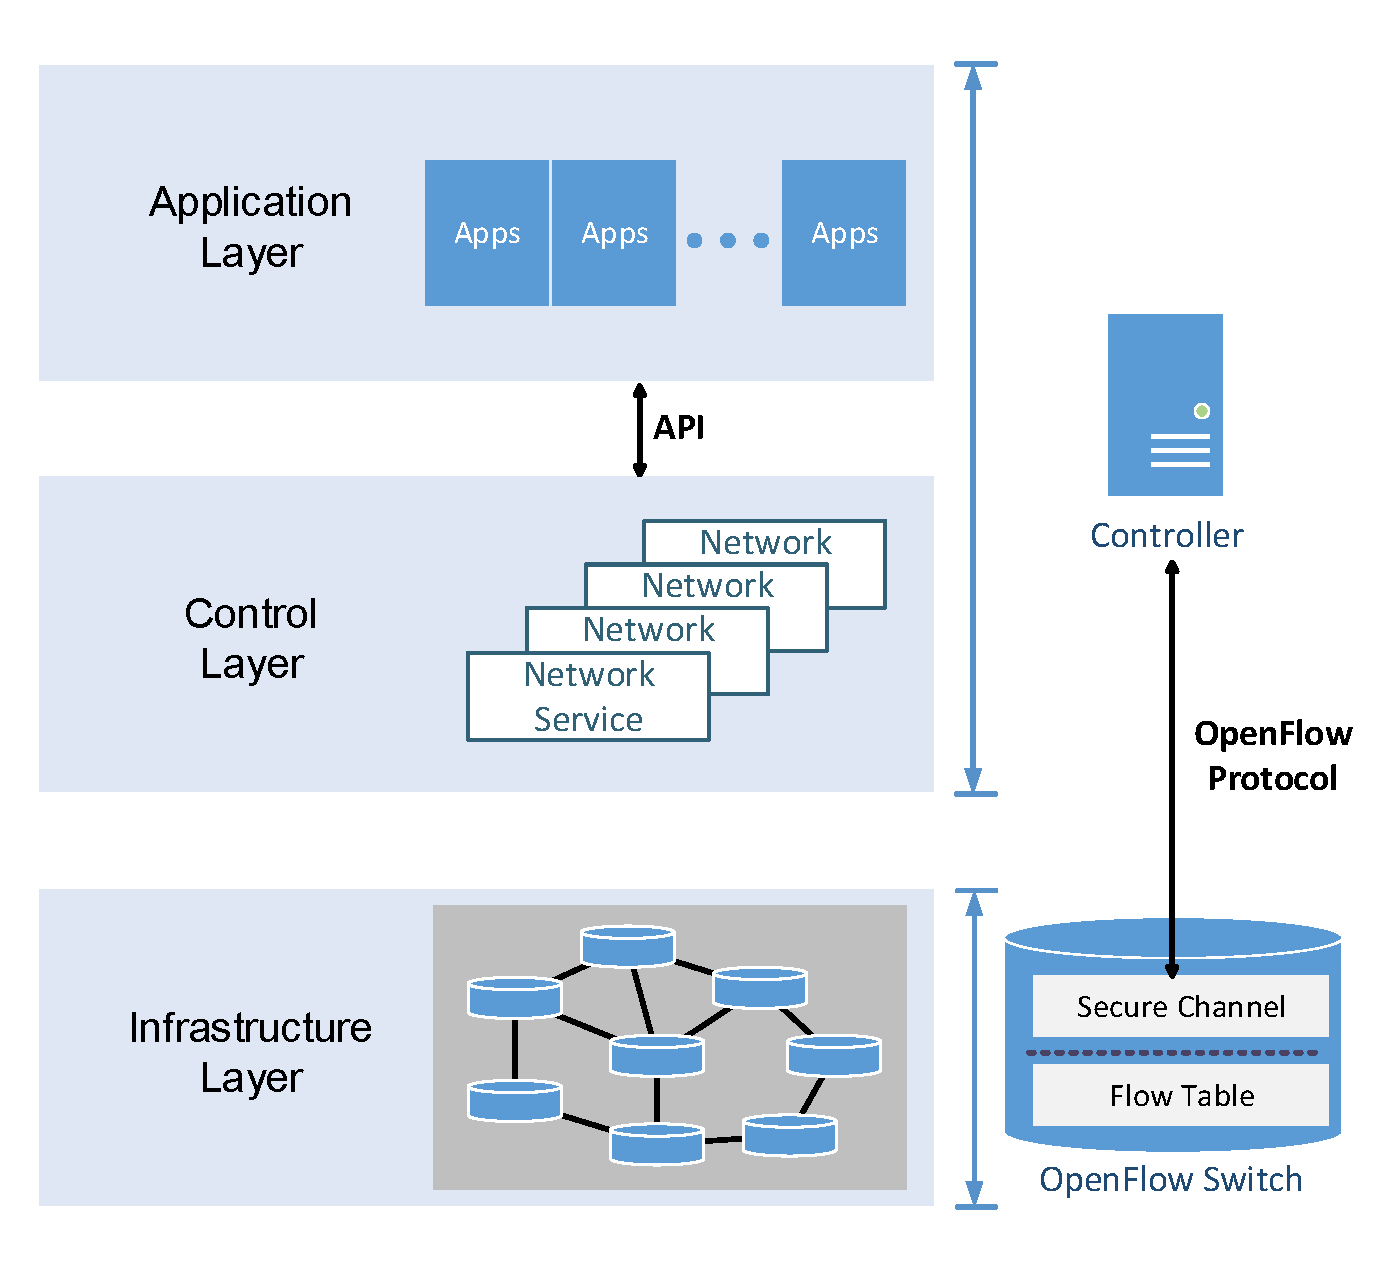
\includegraphics[width=3.4in]{images/SDN_architecture.pdf}
% \end{center}
% \caption{SDN Architecture}
% \label{fig:SDN-Architecture}
% \end{figure}
%\clearpage

% The Stanford University proposed a wireless SDN platform in Clean Slate plan, called “OpenRoads” \cite{yap2010openroads}. It is built on OpenFlow and SNMP, so it allows researchers to design mobility management mechanism by changing the forwarding rule or controlling the wireless AP configurations. For example in \cite{kim2014seamless} and \cite{dely2013software}, the issues of handover and performance anomaly are discussed based on SDN. The approach of OpenRoads project shows that continued innovation and development in wireless SDN can be expected.



% \subsection{Association Control}
%In this section, we introduce some existing user-to-AP association decision schemes which were proposed to balance the total AP load. 
In this section, we describe existing association control schemes and load balancing schemes in literature.
% which are based on association control.
%We classify these schemes into three categories: \emph{strongest signal first} (SSF), \emph{least load first} (LLF) and \emph{Cell Breathing}.

%\begin{itemize}
%	\item SSF: 
The strongest signal first (SSF) method is the traditional association mechanism defined in IEEE 802.11 standards~\cite{ieee2001ieee}. 
	%If a user has many APs to choose, it will select the AP with the largest Received Signal Strength Indicator (RSSI) value to associate with.
	When a device detects more than one AP, the device selects the AP with the largest received signal strength indicator (RSSI) value for association.
%	In \cite{teng2009d} and \cite{wu2007proactive}, user are setting to re-associated with the stronger signal strength AP. 
This method is also widely adopted in handoff schemes~\cite{teng2009d,wu2007proactive}.
	The main problem of these schemes is the load imbalance of APs. 
	When too many users associate to an AP with strong signal at the same time, these users may incur worse performance from the overloaded AP.
	
%	\item LLF: 
	Least load first (LLF) is the most straightforward load balancing scheme, where users select the  AP with least number of users~\cite{papanikos2001study}.
	% proposed an association metrics by considering the number of users currently associated with AP. 
	In~\cite{balachandran2002hot}, Balachandran et al. proposed 
	%an association selection scheme 
	that users associate to the AP which can provide sufficient bandwidth based on the users' bandwidth requirement. 
	In \cite{bejerano2004fairness}, Bejerano et al. further consider the fairness among all users in  association control.

%	\item $\emph{Cell Breathing}$: 
The cell breathing concept has been studied mostly in code devision multiple access (CDMA) cellular network. 
In \cite{bahl2007cell} and \cite{bejerano2009cell}, cell breathing was applied to IEEE 802.11 WLANs. 
Figure \ref{fig:cell-breathing} illustrates an example of cell breathing method. 
First, the three APs in Figure~\ref{fig:fig2_2a} are associated with 1, 7, and 1 users, respectively.
Through adjusting the power levels of APs, some users of AP b shift to adjacent APs, and then the APs are all associated with three users in Figure \ref{fig:fig2_2b}. 
In the cell breathing method, an access controller can obtain the load of APs, but 
it has no information of users' positions. 
In this case, the controller can only adjust the beacon power of the AP with the highest load step by step until the load of APs is balanced.
%For the related work of cell breathing method, 
To achieve load balancing, in \cite{bejerano2009cell}, Bejerano et al. proposed an algorithm to determine globally optimal inter-AP fairness. 
However, both \cite{bahl2007cell} and \cite{bejerano2009cell} 
adjust the AP power level based on limited information (e.g., number of users).
%cannot adjust the AP power level adaptively due to limited information of AP loads. 
% without any prediction of association change trend.
%\end{itemize}

%% Fig:2.2
\begin{figure}
	\centering
		\subfigure[All APs have the same power level.]
		{
			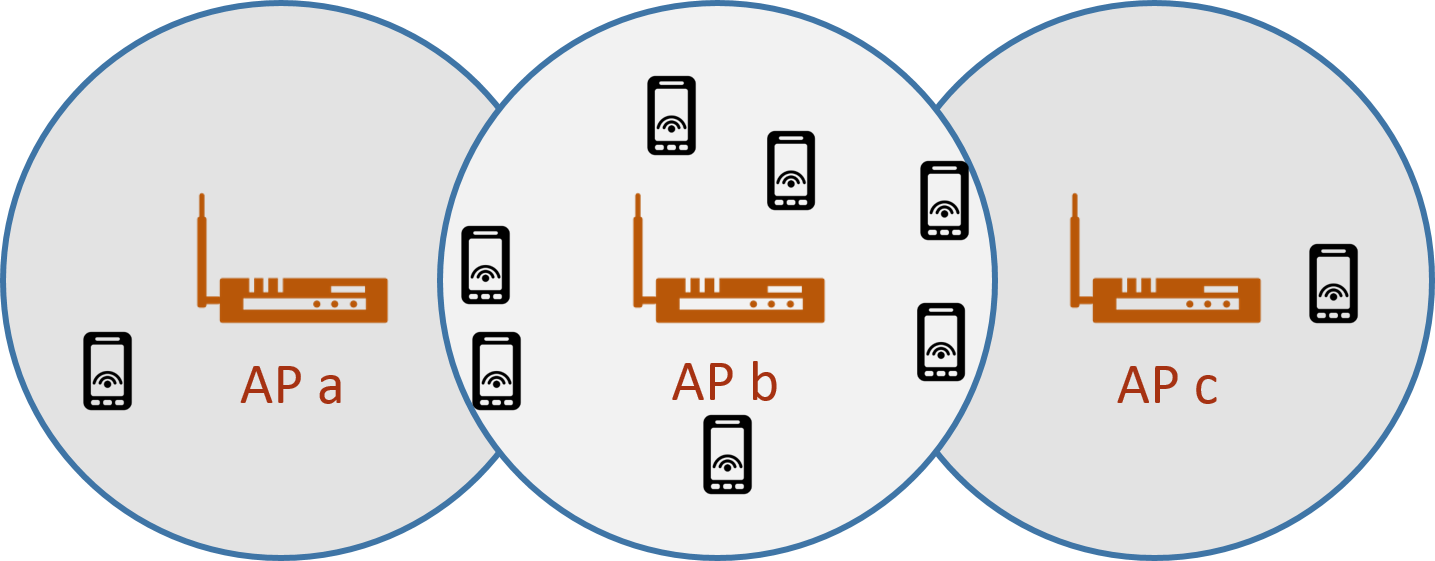
\includegraphics[scale=0.23]{images/cb_before.png}
			\label{fig:fig2_2a}
		}
		
		\subfigure[ AP $b$ transmits with the lowest power level.]
		{
			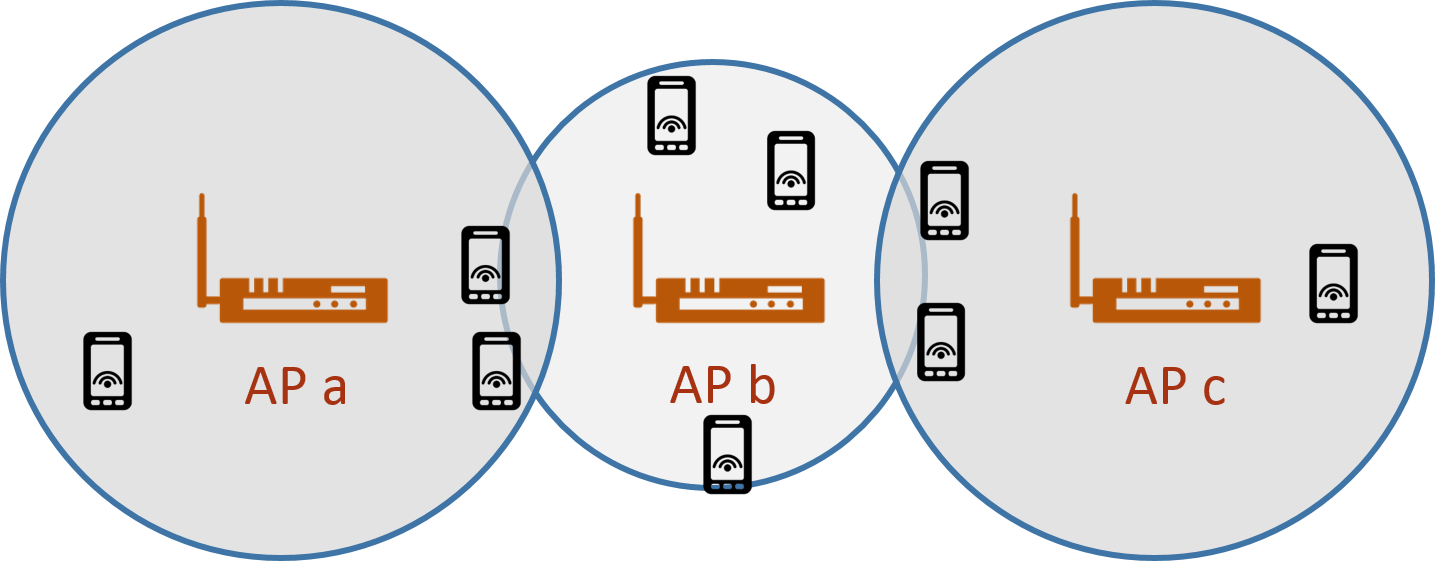
\includegraphics[scale=0.23]{images/cb_after.png}
			\label{fig:fig2_2b}
		}
		
	\caption{Using Cell Breathing Method for Imbalanced Situation.}
	\label{fig:cell-breathing}
\end{figure}

In this paper, we propose an adaptive load balancing scheme which can further improve performance of
%by combining the 
cell breathing by considering the flexibility of SDN.
% method with SDN. 
Through SDN, we can use the global vision to collect the load of AP and users' RSSIs accurately. 
%In this way, our scheme is adaptive. 
Furthermore, the users' positions can be derived by users' RSSI according to~\cite{zaruba2007indoor}. 
% above Dotto



\section{Proposed Scheme} \label{ch:3-proposed}
	%\hspace{24pt}


\subsection{System Model}\label{section:3.1}
% ==== Transfrom table from image to latex by little six 2016/10/14====
%%Table1
% \begin{table}[tbp]
% \setlength{\belowcaptionskip}{15pt}
% \centering
% \caption{Notations}
% \label{tab: Notations}
% 
\includegraphics[width=3.4in]{images/notations.png}
% \end{table}

\begin{table}[tbp] 
    \normalsize
    \caption{Notations} 
    \begin{center} 
        \label{tab: Notations} 
        \begin{tabularx}{\linewidth}{| c | X | } 
            \hline \textbf{Symbol}  & \textbf{Semantics} \\ 
            \hline $A$              & the set of all access points (APs) \\ 
            \hline $U$              & the set of all users \\ 
            \hline $U_a$            & the set of users associated with AP $a$, $a \in$ \{1, 2, ..., $|A|$\} \\ 
            \hline $L_a$            & the load of AP $a$ \\ 
            \hline $L_{a,u}$        & the load contribution of user $u$ to AP $a$ \\ 
            \hline $C$              & the set of overcrowding APs \\ 
            \hline $P_a$            & transmission power of AP $a$\\ 
            \hline $P_{a, max}$     & the maximum transmission power of AP $a$\\
            \hline $P_{a, min}$     & the minimun transmission power of AP $a$\\
            \hline $P^{*}_{a}$      & the transmission power level of AP $a$\\
            \hline $N$              & the number of transmission power level\\
            \hline $P^{*}_{a(lv.n)}$   & the transmission power level of AP $a$ at level $n$, $n$ $\in$ $[$0, $N]$\\
            %%  ==== comment by little six 2016/10/21 ==== 
            %%  (equation 1 would explain this)
            %, $P^{*}_a$ = $log_\gamma P_a$ \\ 
            \hline $S_v, S_n, S_o$  & three different load level set of APs, $A$ = $S_v$ + $S_n$ + $S_o$ \\ 
            \hline $b_{vn}, b_{no}$ & boundaries between three load state \\ 
            \hline $R_u$            & the RSSI value of user $u$ \\
            %%  ==== comment by little six 2016/10/21 ==== 
            %%  (not used in following description)
            % \hline $TH_{lq}$        & RSSI threshold within Section low quality (LQ) and acceptable quality (AQ) \\ 
            \hline $S^k$            & the network states during a load-balancing process\\
            %%  ==== comment by little six 2016/10/21 ==== 
            %%  (different definition of N)
            %, k $\in [$0, $N]$ \\ 
            \hline 
        \end{tabularx} 
    \end{center} 
\end{table}

Figure \ref{fig:scheme1} shows our system architecture. 
The notations used in our scheme are shown in Table \ref{tab: Notations}. 
We consider an IEEE 802.11 WLAN with a set of APs, which is denoted by $A$, and $|A|$ indicates the number of APs. 
All APs are attached to a wired infrastructure and an OpenFlow controller. 

In our scheme, we focus on the transmission power of AP beacon messages since beacon messages are used for AP association.
% to the AP selection of users. 
We denote transmission power of AP $a$ as $P_a$.
According to the configuration and ability, each AP has its maximum and minimum transmission power, denoted as $P_{max}$ and $P_{min}$ respectively. 
Each AP also provides several transmission power levels from $0$ to $N$, denoted by $P_{a(lv.n)}^*$. 
We denote $P_{a(lv.0)}^*=P_{a, min}^*$ as the minimum power level of AP, and similarly we denote $P_{a(lv.N)}^*=P_{a, max}^*$ as the maximum power level.
For normal commercial AP products, the transmission power level configuration follow that
%We define 
\begin{eqnarray}
{P_a^*}=log _\gamma\left({P_a} \right)  \quad,\gamma=\sqrt[N]{\frac{P_{max}}{P_{min}}}
\end{eqnarray}
Then $P_{a(lv.n)}^*$ is a geometric series which can be expressed as
\begin{align}
&P_{a(lv.k)}^*={P_{a(lv.k-1)}^*}*\gamma\\										
&P_{a(lv.k)}^*={P_{a, min}^*}*{\gamma^k}, k\in[0, N].							
\end{align}
In our scheme we have some assumptions. First, we assume that the interference between adjacent cells can be ignored. Second, we assume that the AP deployment ensures complete overlaps between the ranges of all APs. In other words, if all APs are configured to the minimum transmission power $P_{min}$, every user in network coverage area can be still covered.

When a mobile device joins a WLAN, it listens every channel for all beacon messages from APs. Then, it associates with an AP which has the strongest RSSI, which is determined by the beacon transmission power and the distance between AP and user. In our system, we use all APs to collect the RSSIs from users  (Figure \ref{fig:scheme1}). Each AP reports the RSSIs to the controller by using OpenFlow protocol. Once in a while, each AP collects its load $L_a$  and the load contribution of its users $L_{a,u}$  to controller. Based on the information above, the controller knows the association relationships between users and APs. In the same way, the load of APs is also known by controller. In our system, the controller has a global view of the whole network.

We use $U$ to denote the set of all users in the network coverage area and $|U|$ is total number of users in U. Each user associates with at most one AP at any time, and we denote $U_a$ as the set of users associated with AP $a$. In normal cases, if a large amount of user association requests are sent to an AP in a short time, the AP become overloaded seriously. To stress the coordination ability of APs, we consider the group arrival cases. We assume that all users follow a group mobility model in our system. The users usually move together from one place to another in several groups.

Owing to the global vision of controller, we design an adaptive load balancing model using association allocation. Our model can coordinate the load of all APs and take the users' load contributions into consideration. For example, the busy users, who need whole allocated bandwidth to upload or download data frequently, are considered. The controller records the load contribution of user $u$ to AP $a$, $L_{a,u}$ by considering the load report from APs. Each AP can provide different bandwidths to its associated users in our case.

%% Figure 3.1

\begin{figure}[tbp]
\begin{center}
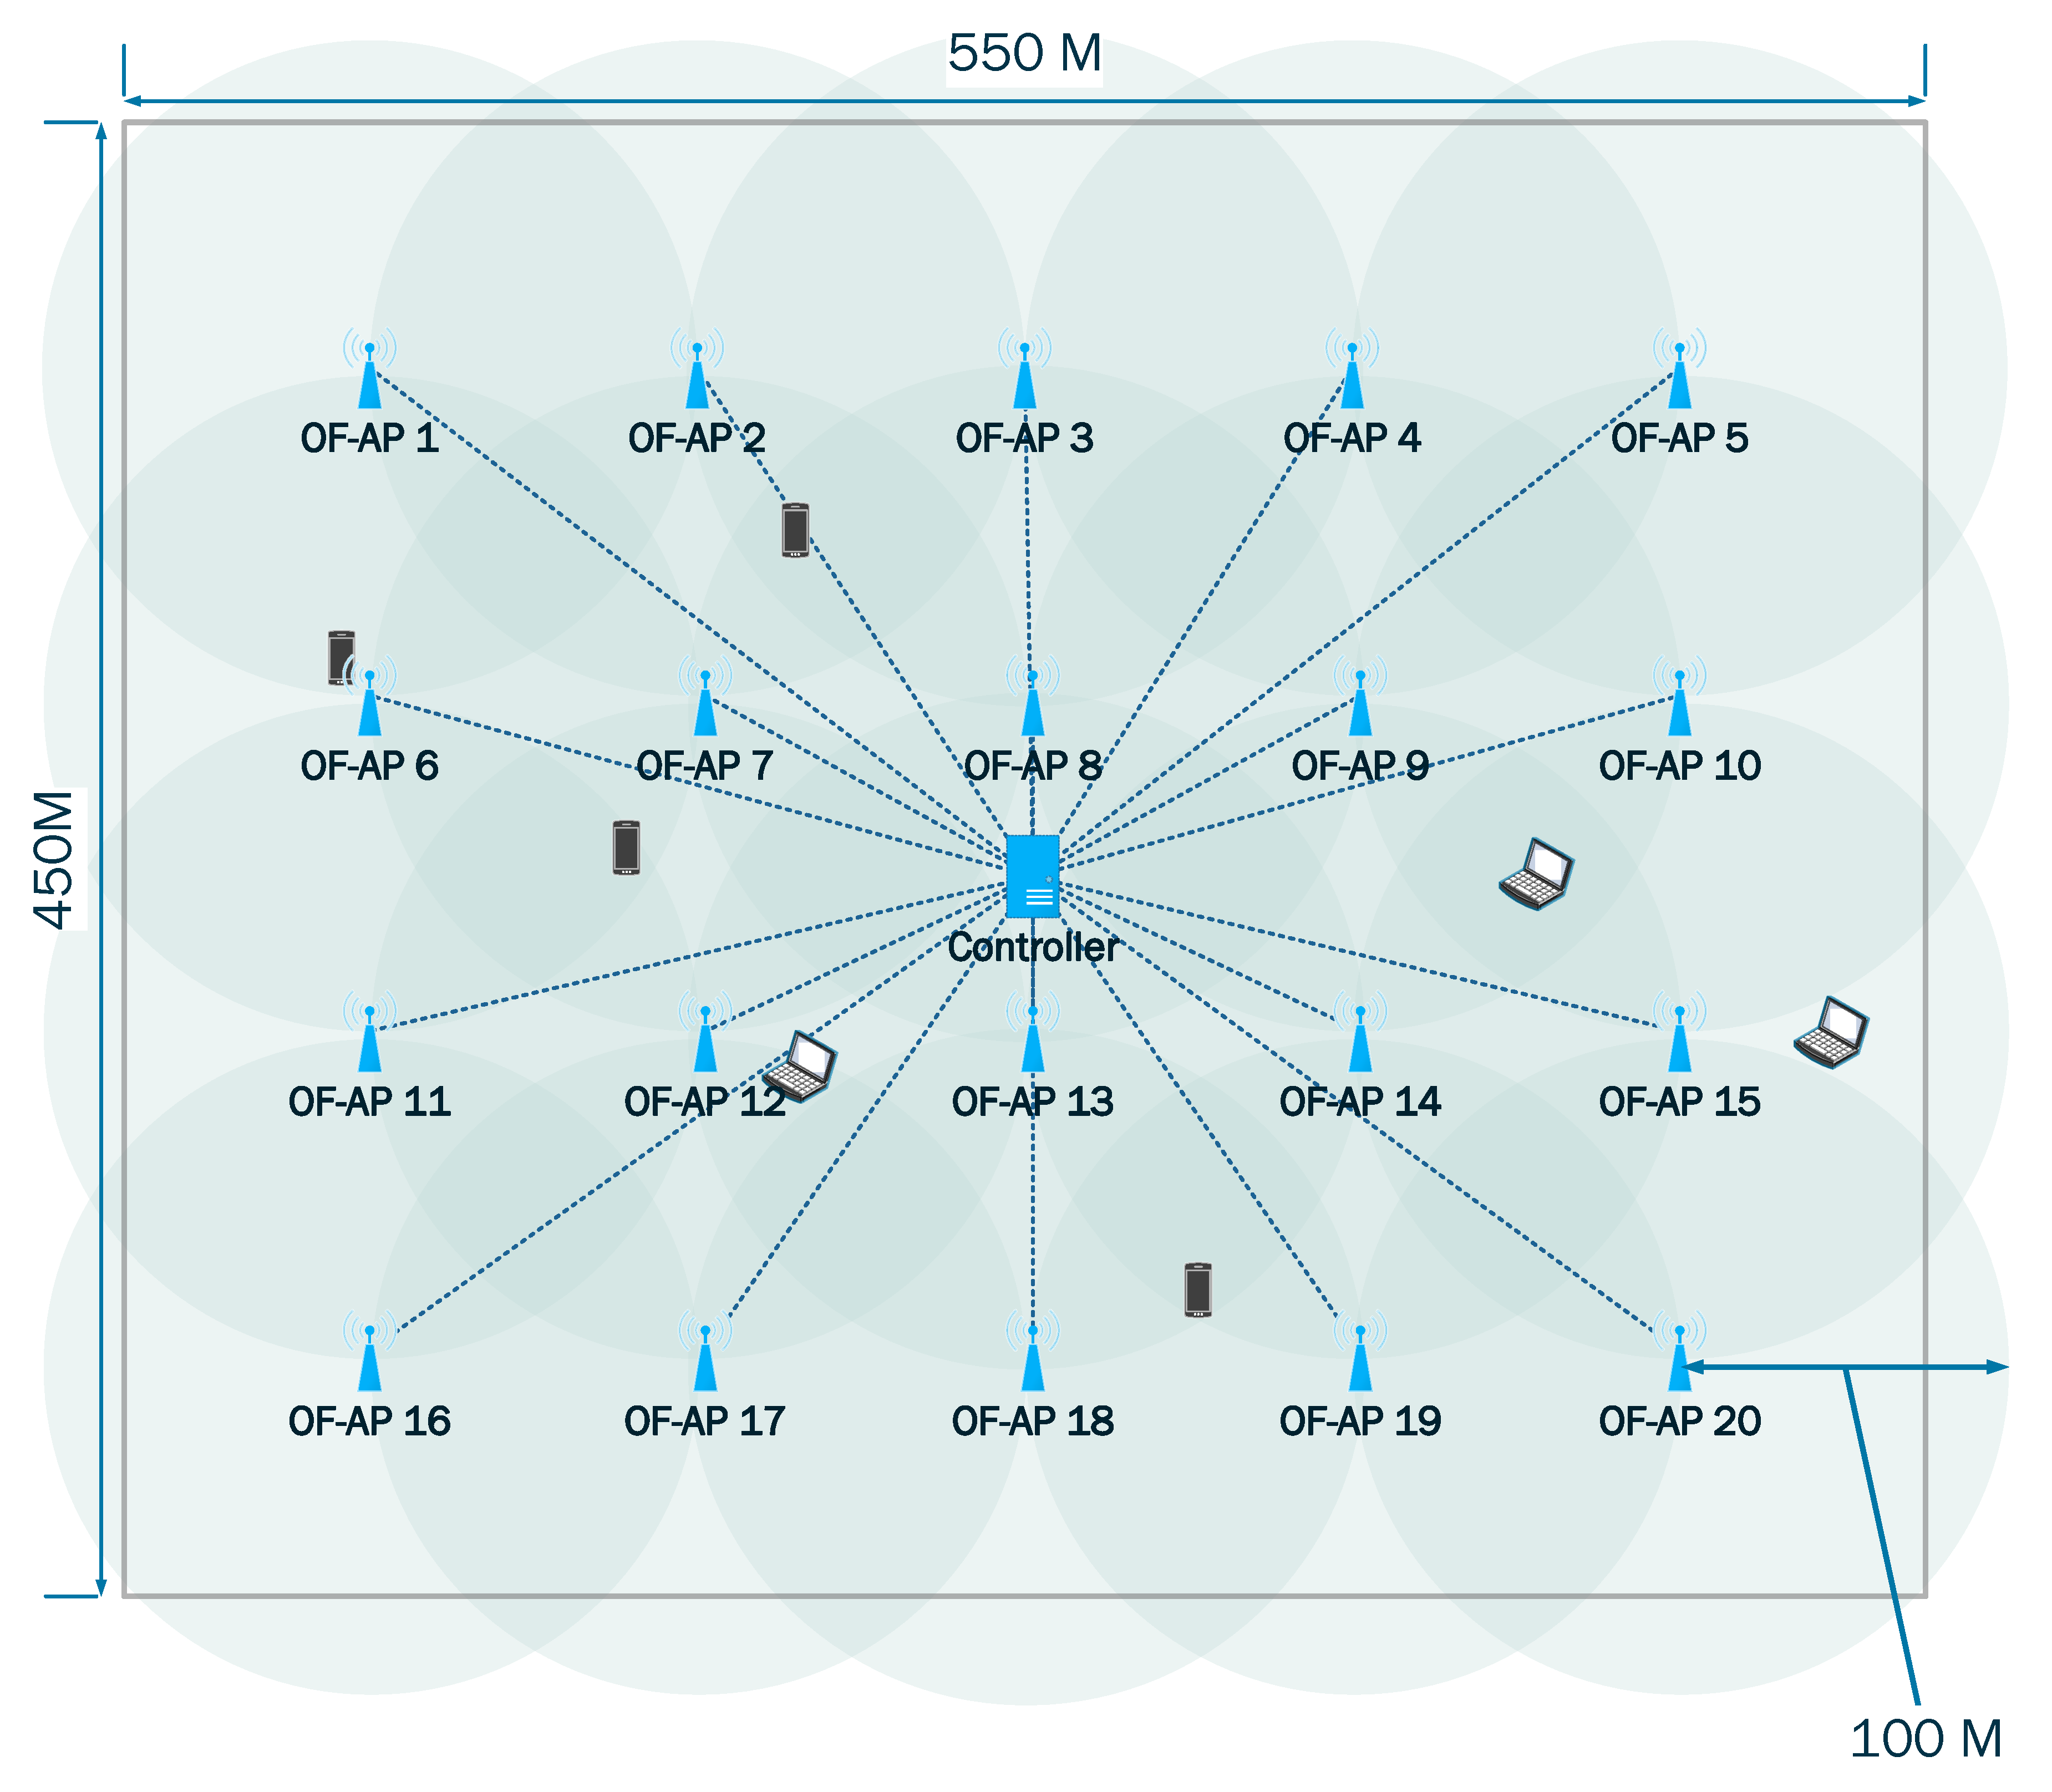
\includegraphics[width=3.4in]{images/scheme1.pdf}
\end{center}
\caption{System Architecture}
\label{fig:scheme1}
\end{figure}
%\clearpage

\subsection{Arrival Event Detection}\label{section:3.2}
In this subsection, we present the initial stage of adaptive load balancing. We design the procedures for APs to report its user association events and load in real time. Figure \ref{fig:flowdiagram_trendindicator_ap} shows the flow chart of AP reporting mechanism, and the steps are described below.

\begin{description}
  \item [Step 1.] Each AP records the user RSSI, user association list and its load periodically. All APs receive RSSIs in every authentication frames from their users.
  \item [Step 2.] If there is a new user associating with the AP, go to \textbf{Step 3}. Otherwise, go to \textbf{Step 4}.
  \item [Step 3.] The AP sends the user RSSI to the controller. Then go to \textbf{Step 6}.
  \item [Step 4 and 5.] If there is no new arrival in \textbf{Step 2}, the AP reports its load to controller periodically.
  \item [Step 6.] After sending report messages to controller, the AP would receive a Beacon-Config message from the controller.
  \item [Step 7.] The AP configures its beacon transmission power.
\end{description}

%% Figure 3.2
\begin{figure}[tbp]
\centering
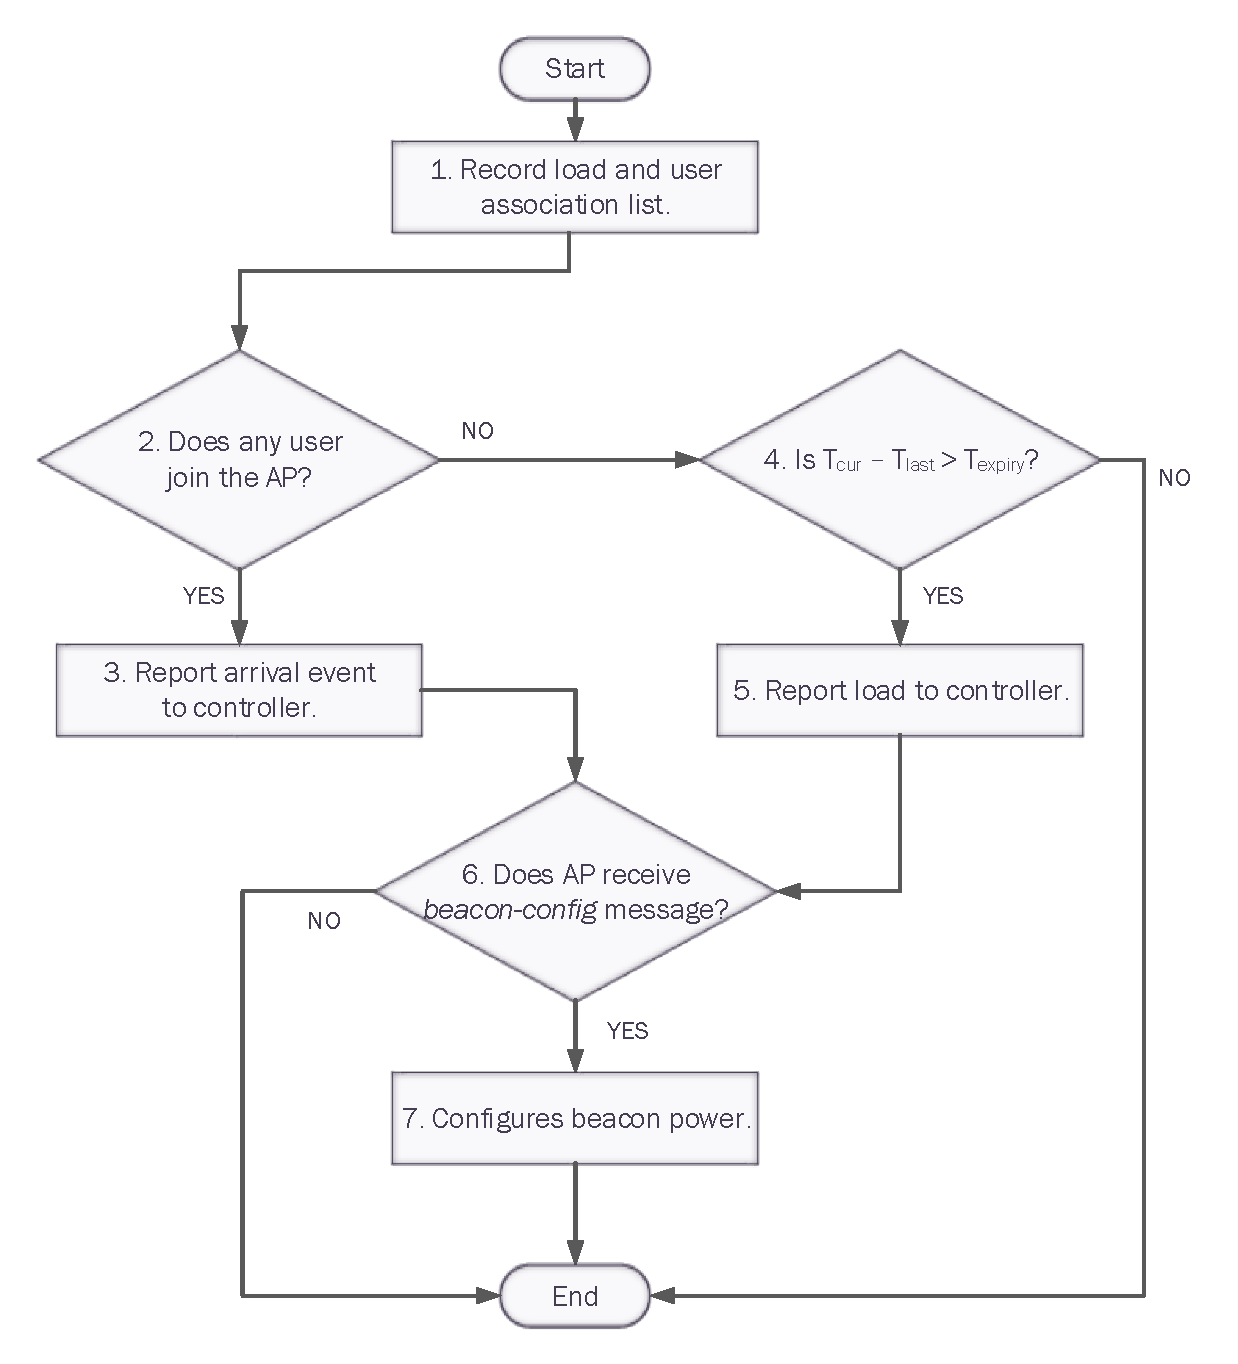
\includegraphics[width=3.4in]{images/flowdiagram_trendindicator_ap.pdf}
\caption{Flow Chart for AP Reporting Mechanism}
\label{fig:flowdiagram_trendindicator_ap}
\end{figure}

%\clearpage
% comment out by little six 2016/10/14
%On the other side, we describe a flow chart of controller manage mechanism in Figure \ref{fig:flowdiagram_trendindicator_controller}.
The flow chart of the controller management mechanism is shown in Figure \ref{fig:flowdiagram_trendindicator_controller}, and following is the descriptions of steps.

\begin{description}
  \item [Step 1.] The controller receives arrival events and load messages from APs.
  \item [Step 2.] The number of new arrival events is added into the arrival counting table. Then the controller calculates event increase at the latest time interval.
  \item [Step 3.] The controller compares the number of current arrival events with the past. When an AP exceeds the threshold of arrival events, it has a high risk of overcrowding. At this time, the controller gives the AP a predicted load value and then go to \textbf{Step 6}.
  \item [Step 4.] The controller classifies all APs into three load levels: vacant, normal and overcrowding. According to the levels, the APs are added into $({S_v}$, ${S_n}$ and ${S_o}$) respectively. The $b_{vn}$ and $b_{no}$ denote the boundaries between these levels.

      \begin{align}
        &L_{l,a}=\left\{\begin{array}{lll}
            v, L_a \leq b_{vn} \\ n, L_a \leq b_{no} \\ o, L_a < b_o
            \end{array} \right\} \\
            \nonumber\\
        &S_v={a|L_{l,a}=v}\\
        &S_n={a|L_{l,a}=n}\\
        &S_o={a|L_{l,a}=o}
      \end{align}
  \item [Step 5.] This procedure ends when there is no AP changing to overcrowding state $S_o$.
  \item [Step 6.] The controller calculates the adjustments of APs according to the load balancing algorithm which is described in next subsection.
  \item [Step 7.] The controller send a beacon-config messages to each AP.
\end{description}

%% Figure 3.3
\begin{figure}[tbp]
\begin{center}
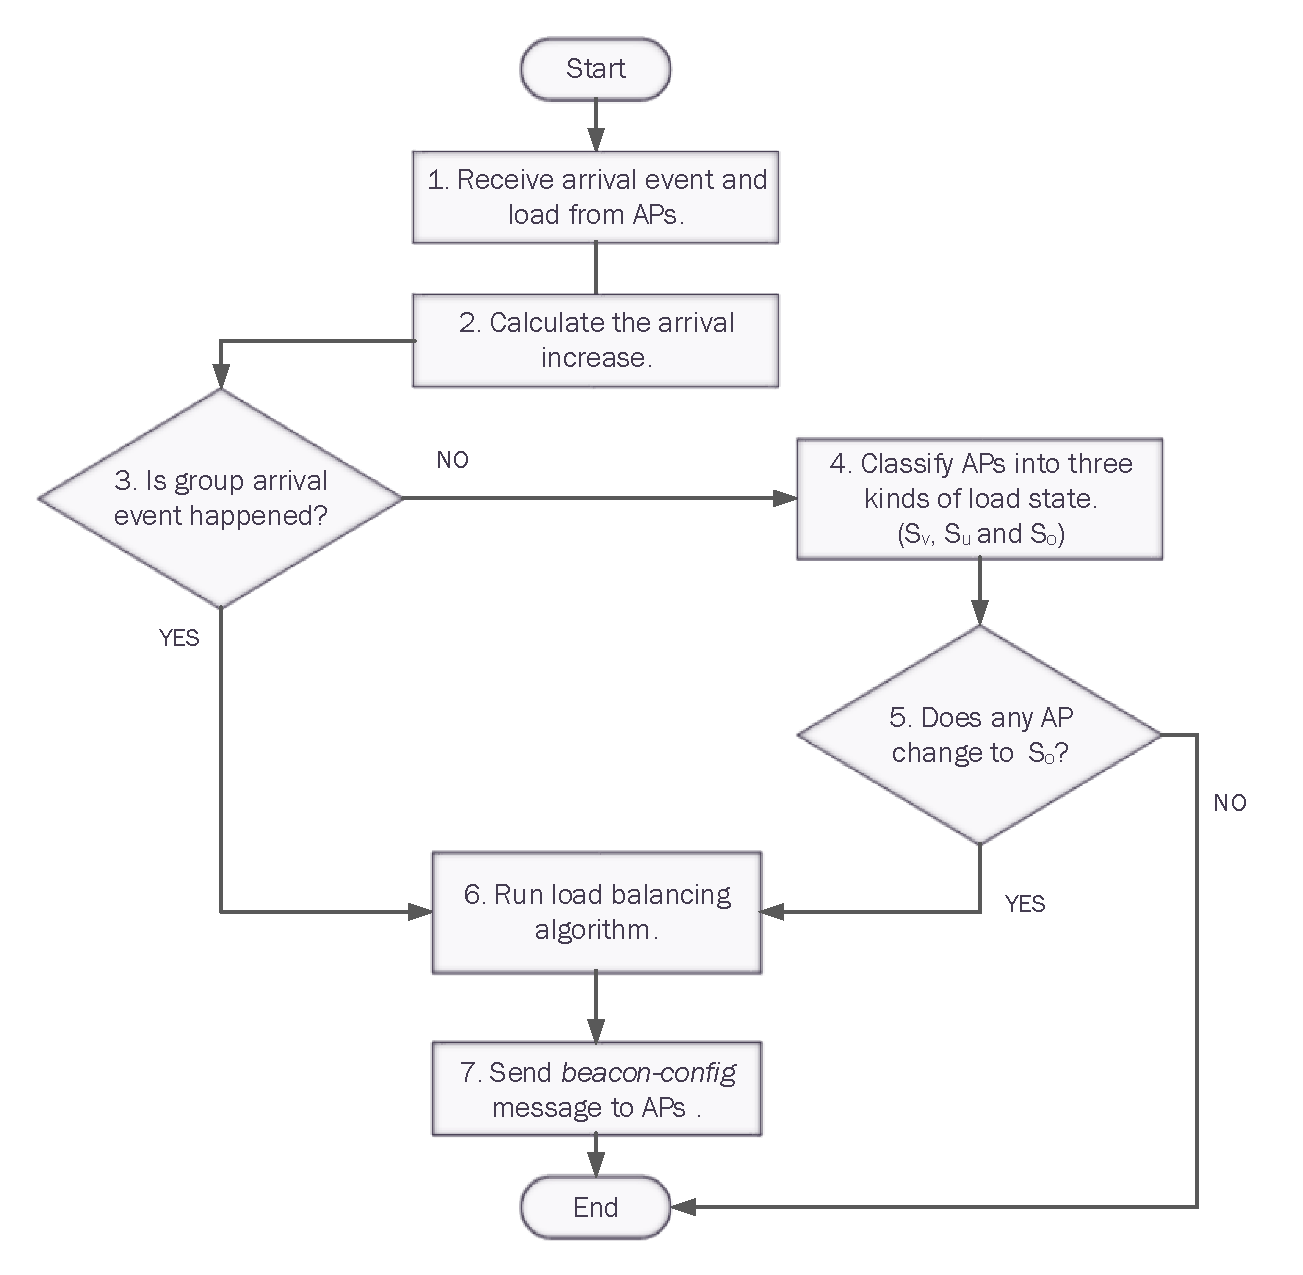
\includegraphics[width=3.4in]{images/flowdiagram_trendindicator_controller.pdf}
\end{center}
\caption{ Flow Chart for Controller Management Mechanism}
\label{fig:flowdiagram_trendindicator_controller}
\end{figure}
%\clearpage

\subsection{Adaptive Load Balancing}
In this subsection, we present the adaptive load balancing mechanism. Recall what we described in subsection \ref{section:3.1} and \ref{section:3.2}, the association relationship, RSSIs of users and load of APs are all collected by the controller. Based on the information above, the controller has a global vision of whole wireless network. We combine SDN and Cell-Breathing method into an Adaptive Load Balancing mechanism.

 Figure \ref{fig:algorithm} shows the pseudo code of our mechanism for controller. In this algorithm, the beacon power level is first initialized to the maximal power level. The controller collects and calculates the summations of all AP utilizations, and the network state is initialized as $S^0$. First, the algorithm iteratively finds the most overcrowding AP, then set its power one level down. In the meanwhile, the adjustment is recorded in a stack structure and the most overcrowding AP is added into overcrowding set $C$. Every time the most overcrowding AP sets down beacon power level, the algorithm updates the AP states by simulating the association relationship between APs and users. Each state is compared with previous states to find the optimal state. Until the iteration ends, the algorithm sets all AP beacon power level according to the optimal state.

This algorithm terminates in two conditions. The first condition is that the overcrowding set $C$ is equal to AP set $A$. When these two sets are equal, every AP is adjusted. At this time, the results are the same, even though the iteration continues. The second condition happens when any AP beacon power level is zero. If the iteration continues, some APs can not trun down their beacon power anymore, thus they become overcrowding again.

%% Algorithm
\begin{figure}[tbp]
\centering
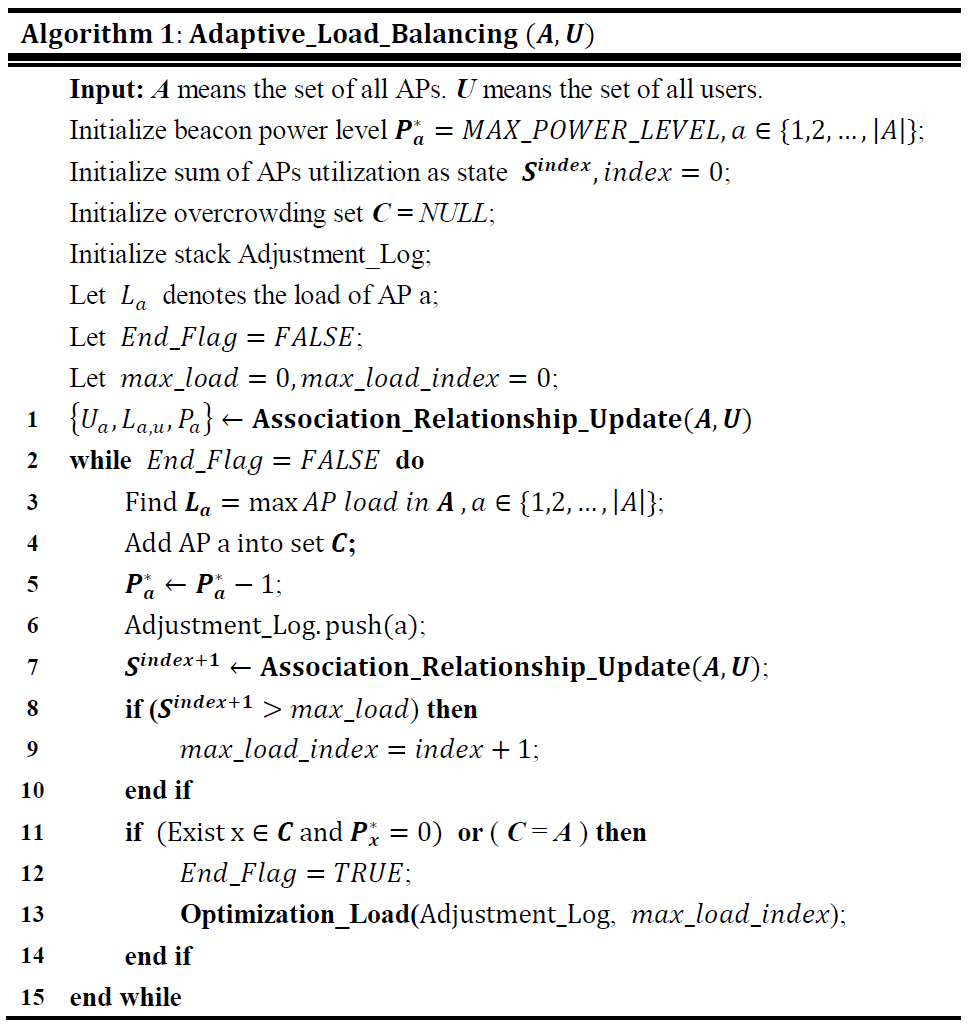
\includegraphics[width=3.4in]{images/algorithm.png}
\caption{Adaptive Load-Balancing Algorithm}
\label{fig:algorithm}
\end{figure}
%\clearpage

Figure \ref{fig:flowchart_Cell_Breathing} illustrates the message flow of association control between users, APs and controller. We assume that user is in the coverage of AP 1 and 2, and AP 1 is closer to user than AP 2. We assume that the user has passwords of AP 1 and AP 2. Both these two APs connect to controller via secure channel.

\begin{description}
  \item [Step 1.] AP 1 and AP 2 send Beacon Message to the user periodly.
  \item [Step 2.] AP 1 and AP 2 report their load (utilization) and association events to controller. In OpenFlow protocol, association event can be transmit in Packet\_In message and the load of AP can be transmitted in Port\_Status message.
  \item [Step 3.] Controller periodly checks all of the AP load and integrates all association event reports of APs. Then controller inputs these information to Adaptive Load Balancing program.
  \item [Step 4.] Based on the result of \textbf{Step 3}, controller sends Beacon-Config messages (i.e. SetConfig message in OpenFlow) to APs. In this case, controller decides to reduce load of AP 1, thus controller sets the AP 1 beacon power lower than AP 2 beacon power.
  \item [Step 5.] The same as \textbf{Step 1}, AP 1 and AP 2 send beacon message to the user.
  \item [Step 7-9.] The user sends association request to AP 2, which has the highest RSSI. After receiving an association response from AP 2, user sends an authentication request to AP 2. When AP 2 sends back authentication response, the connection between user and AP 2 is established.
\end{description}

%% Figure 3.4
\begin{figure}[tbp]
\begin{center}
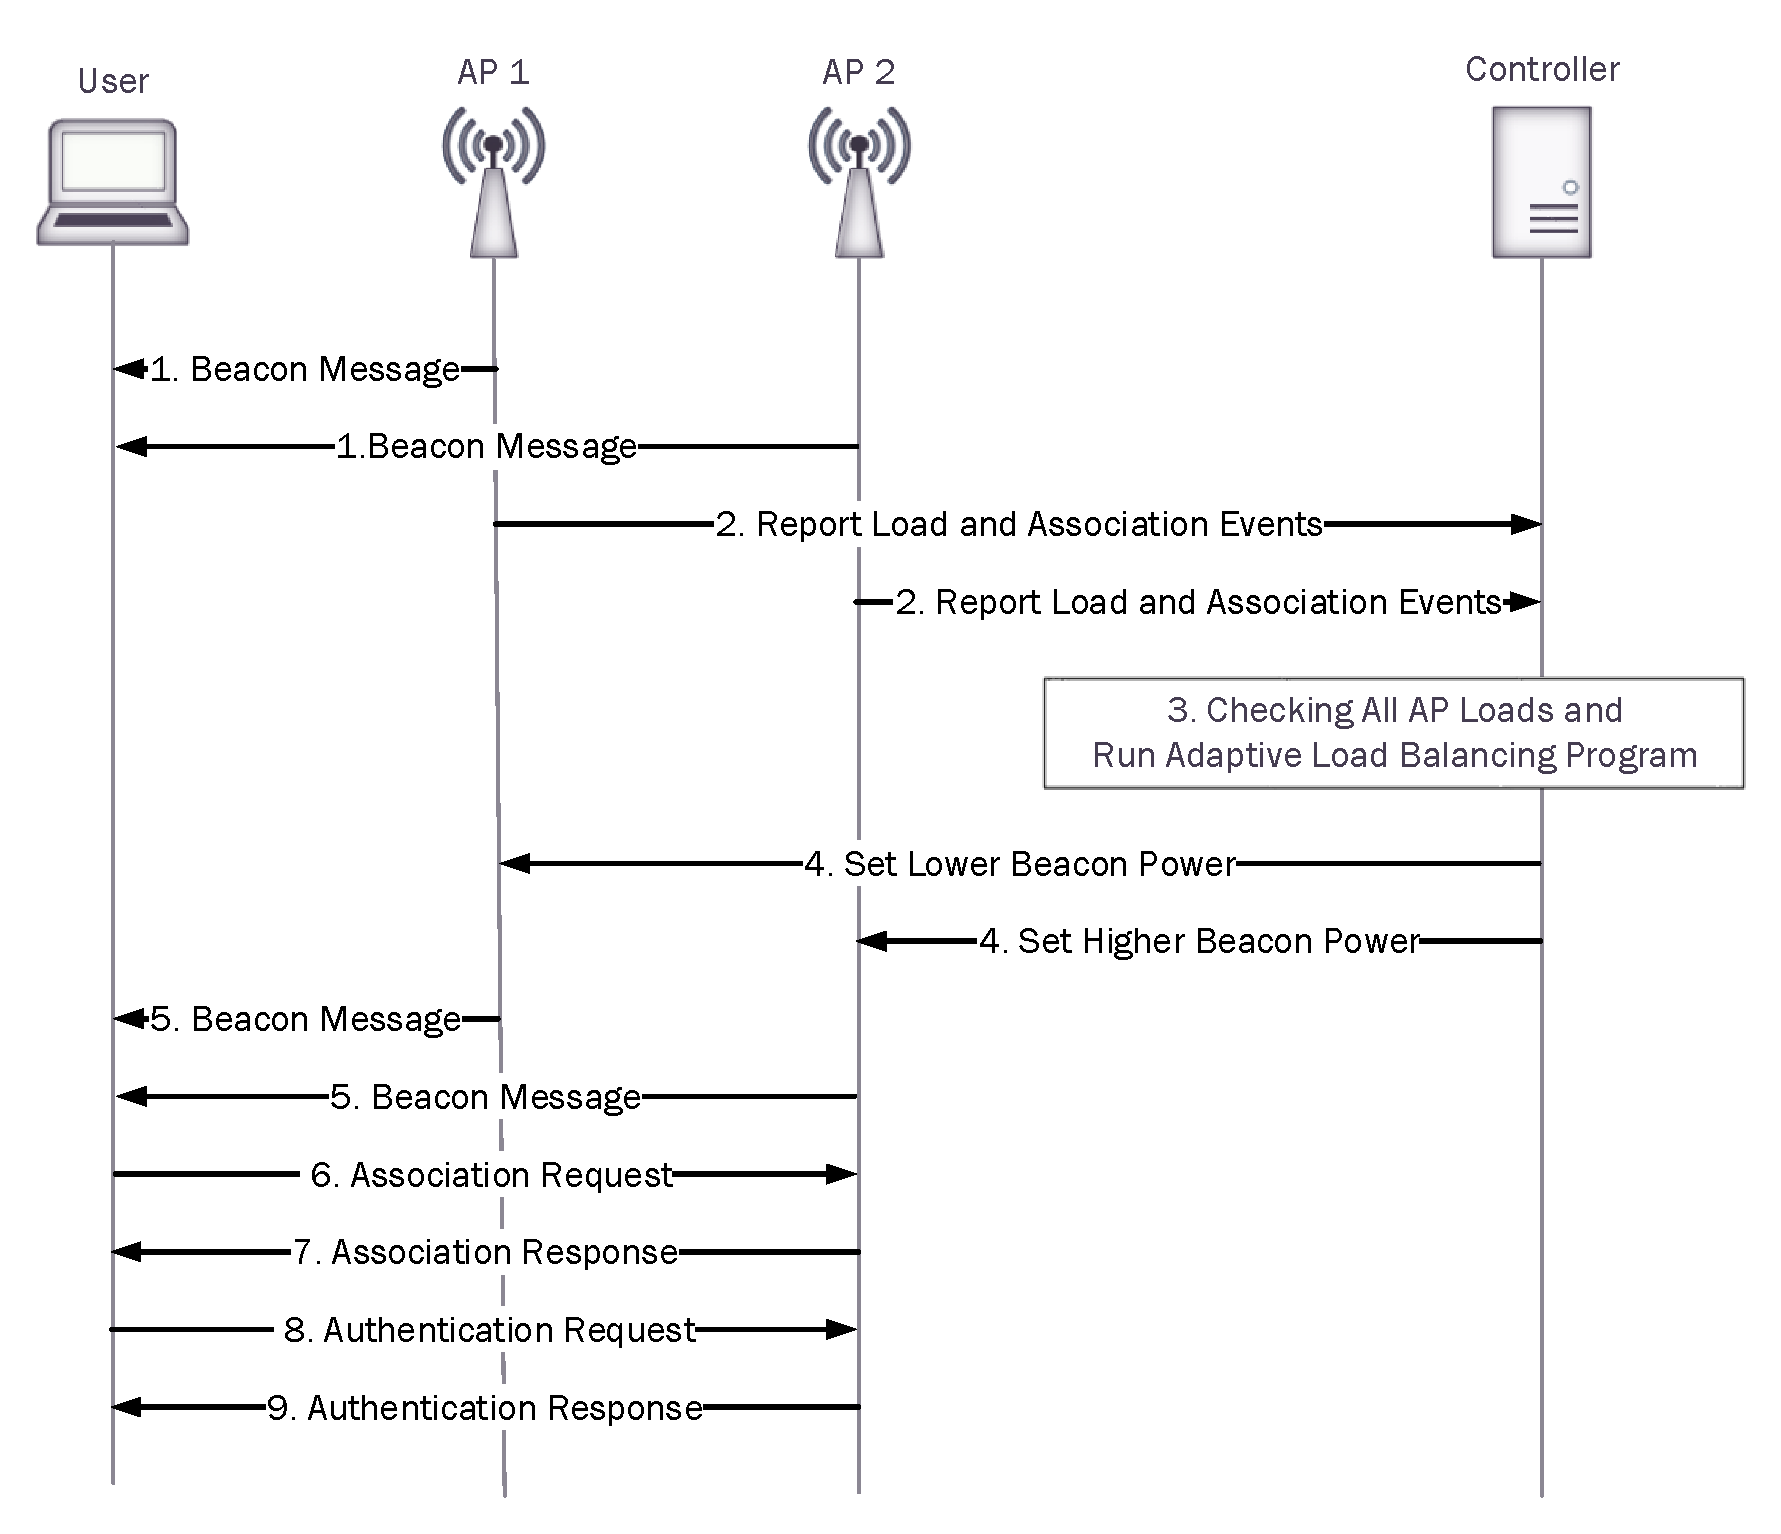
\includegraphics[width=3.4in]{images/flowchart_Cell_Breathing.pdf}
\end{center}
\caption{Message Flow of Association Control}
\label{fig:flowchart_Cell_Breathing}
\end{figure}

% above Dotto



	
\section{Performance Evaluation} \label{ch:5-performance}
	%\hspace{24pt}
In this section, we verify whether our scheme balances the load more significantly than other existing methods including Strongest-Signal-First (SSF), Least-Load-First (LLF) and Cell-Breathing.

\subsection{Simulation Model}
The details of our simulation setup is shown in Table \ref{tab:Simulation-Setup}. Most parameters are configured according to existing Cell-Breathing method in literature \cite{bejerano2009cell}. We use NS3 as our simulation tool, and we set simulation time to 10000s. We totally set 20 APs, which are all support IEEE 802.11g standard. Each AP is equipped with 54 megabits per second backhaul link. These APs are located in $550 * 450 m^2$ area and they are arranged into four lines for five APs per line. The distance between two adjacent APs is set to 100 meters, and those APs are 75 meters far from the simulated area border. In order to ensure that all users are in the coverage of APs, we set the minimum transmission distance is 75 meters. To determine the transmission bit rate between users and APs, we list the relationship between SNR and bit rate in Table \ref{tab:Traffic-Bit-Rate}.

In order to build the mobility of our scenario, we use the BonnMotion tool to generate user traces. We use the Reference Position Group Mobility model (RPGM) to generate three cases of user number, which are 100, 250 and 400. 
%Figure \ref{fig:scenario-400n} shows the scenario with 400 users in our simulated area. 
These users are divided into two groups and follow the group mobility. Each group brings heavy connection demand when the group moves into coverage of an AP.

%% Table 4.1
% \usepackage{booktabs}
\begin{table}[H]
\setlength{\belowcaptionskip}{15pt}
\centering
\caption{Simulation Setup}
\label{tab:Simulation-Setup}
\begin{tabular}{@{}ll@{}}
\toprule
Parameters           & Assumption                               \\ \midrule
Simulated Time       & 10000s                                   \\
Simulated Area       & 550 * 450 m\textasciicircum 2            \\
MAC Protocol         & IEEE 802.11b                             \\
Transmission Range   & {[}75, 150{]} m                          \\
Adjacent AP distance & 100 m                                    \\
AP Number            & 20                                       \\
User Number          & 100, 250,400                             \\
Mobility Model       & Reference Position Group,Mobility (RPGM) \\
Moving Speed         & {[}0.5, 1.5{]} m/s                       \\ \bottomrule
\end{tabular}
\end{table}

%% Table 4.2
% \usepackage{booktabs}
\begin{table}[H]
\setlength{\belowcaptionskip}{15pt}
\centering
\caption{Traffic Bit Rate}
\label{tab:Traffic-Bit-Rate}
\begin{tabular}{@{}ccc@{}}
\toprule
\multicolumn{1}{l}{Bit Rate (Mbps)} & \multicolumn{1}{l}{SNR(dB)} & \multicolumn{1}{l}{Distance (m)} \\ \midrule
11                                  & $\geqq 9$                     & 50                               \\
5.5                                 & $\geqq 5$                   & 80                               \\
2                                   & $\geqq 3$                    & 120                              \\
1                                   & $\geqq 1$                     & 150                              \\ \bottomrule
\end{tabular}
\end{table}
%%\clearpage

%% Figure 4.1
% \begin{figure}[tbp]
% \begin{center}
% 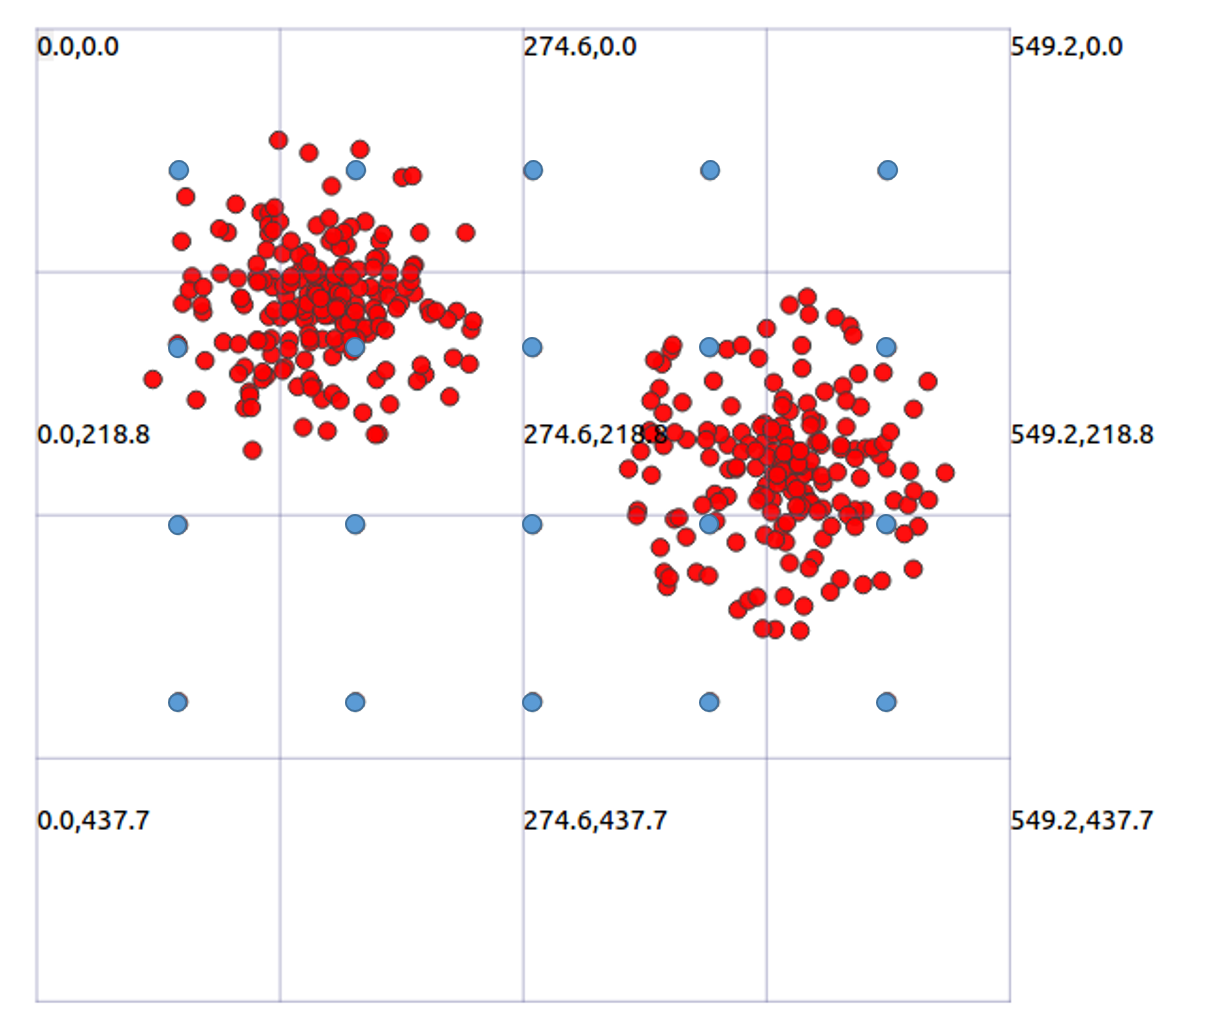
\includegraphics[width=3in]{images/400n.png}
% \end{center}
% \caption{A WLAN Scenario with 20 APs in $550*450m^2$ for NS3 Simulations (The 400 users follow the Reference Position Group Mobility model.)}
% \label{fig:scenario-400n}
% \end{figure}
%\clearpage

\subsection{The Performance of APs}
To measure the performance of APs, we define per second load of AP , $L_a$, to repesent the sum of associated user throughput, $L_{a,u})$. $L_{a,u}$ is the product of user bandwidth and user data rate. We assume the user bandwidth is the time interval that each AP fairly allocates the transmission time slot to its users. Users are able to transmit their data in the time slot. The user data rate can be derived from user SNR or distance with AP in Table \ref{tab:Traffic-Bit-Rate}.
\begin{align}
&L_a=\sum_{u\in{U_a}}L_{a,u}\\
&L_{a,u}=b_{a,u}*r_{a,u}\\
&b_{a,u}=\frac{1}{|U_a|}   ,|U_a|={number\ of\ users}
\end{align}

Figure \ref{fig:fig4_2a}, \ref{fig:fig4_2b} and \ref{fig:fig4_2c} show the average load of all APs with 100, 250 and 400 users respectively. The X-axis represents the index of APs, and the APs are sorted by their average load in increasing order. In the case of 100 users, we generate two groups which have average 50 users. The users are less than 50 meters from their group center. In Figure \ref{fig:fig4_2a}, we notice that the curves of our scheme, LLF and Cell-Breathing are more gently than the curve of SSF. In SSF, some APs are heavily congested and some APs are vacant.  Although the curve of Cell-Breathing is the most gently one, the sum of its average load is the least (in Table \ref{tab:Total-AP-load}). As Table \ref{tab:Total-AP-load} shows, the load of our scheme performs $11\%$ better than SSF and $347\%$ times better than Cell-Breathing. The difference between our scheme and Cell-Breathing is that we consider both the imbalance load distribution and the optimal state of all APs. Limited to the knowledge of network situation, Cell-Breathing is not able to adjust AP beacon power levels to the optimal result.

Figure \ref{fig:fig4_2b} and \ref{fig:fig4_2c} show the curves of our scheme, LLF and Cell-Breathing are more gently than the curve of SSF. In the case of 250 users, we generate five groups which have average 50 users and all users are less than 50 meters near from their group center. In the case of 400 users, we generate two groups which have average 200 users. The users of each group move around the center in 100 meters, and they bring a large amount of connection request to nearby APs. Figure \ref{fig:fig4_2c} illustrates that the gap between SSF and Cell-Breathing is smaller than the gap in Figure \ref{fig:fig4_2b}, and our scheme outperforms these two method.

%% Figure 4.2 (a)(b)(c)
\begin{figure}[tbp]
\setlength{\abovecaptionskip}{0pt}
\setlength{\belowcaptionskip}{0pt}
\begin{center}
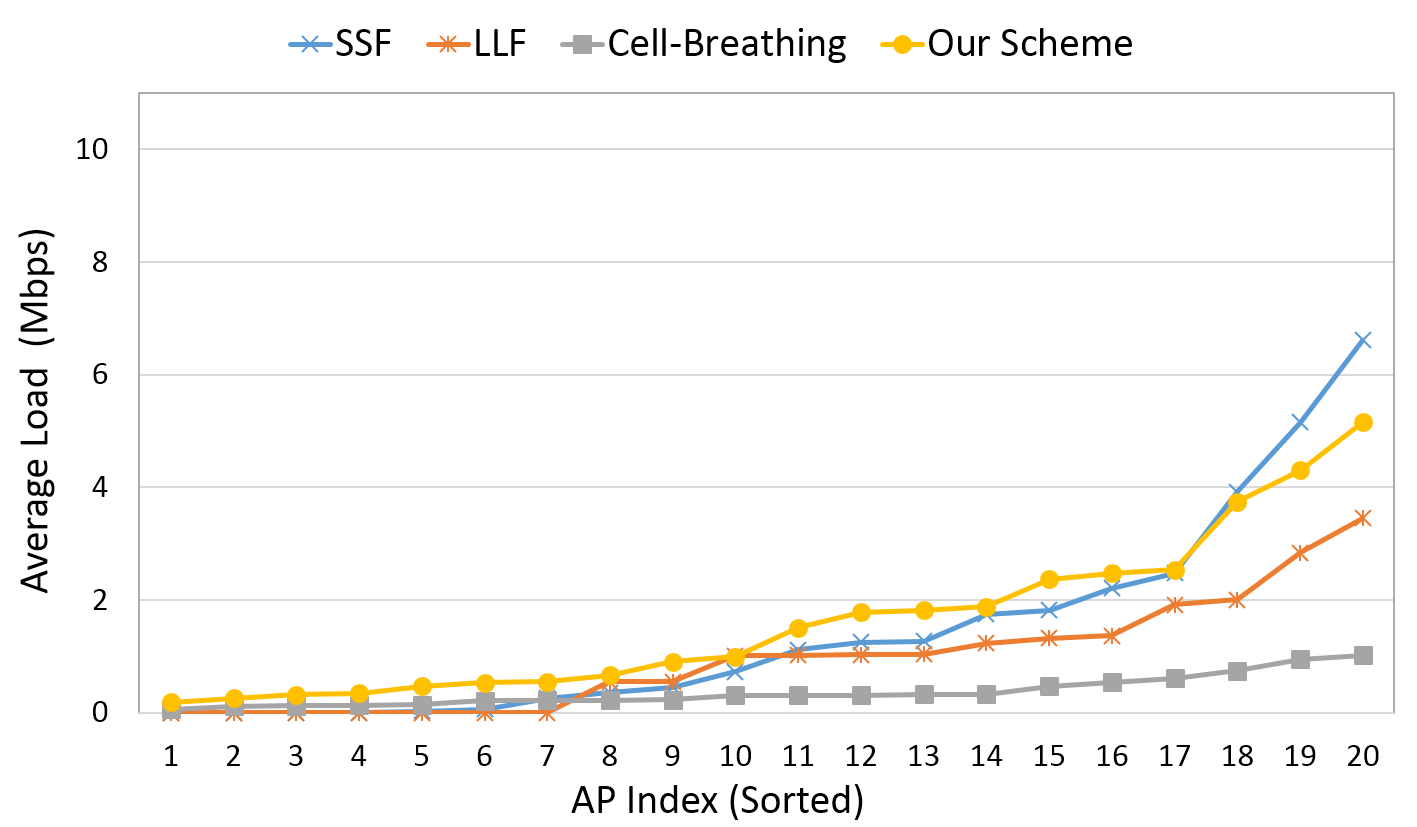
\includegraphics[width=3.4in]{images/Average_AP_load_100.png}
\end{center}
\caption{The Average Load of all APs (100 Users)}
\label{fig:fig4_2a}
\end{figure}

\begin{figure}[tbp]
\setlength{\abovecaptionskip}{0pt}
\setlength{\belowcaptionskip}{0pt}
\begin{center}
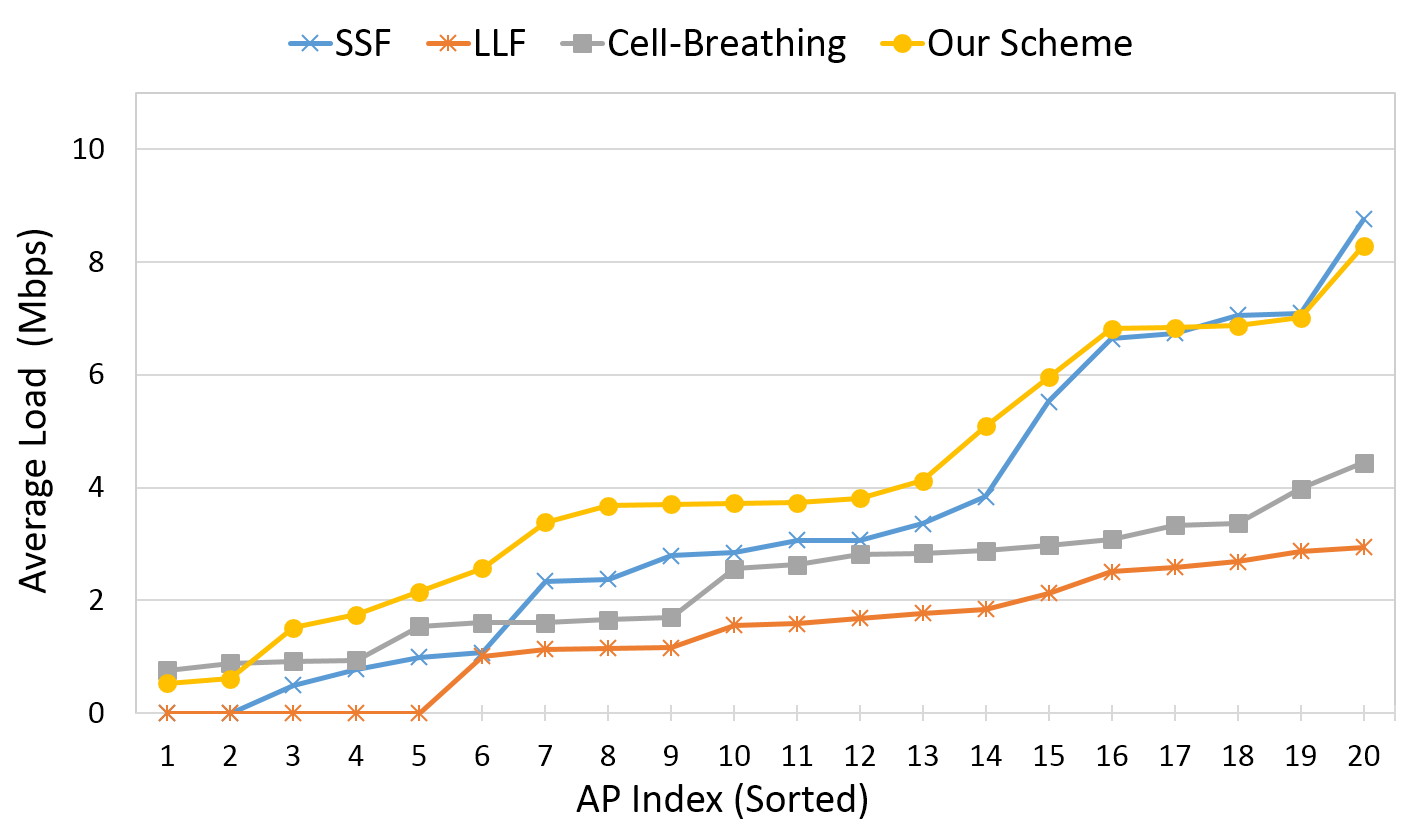
\includegraphics[width=3.4in]{images/Average_AP_load_250.png}
\end{center}
\caption{The Average Load of all APs (250 Users)}
\label{fig:fig4_2b}
\end{figure}

\begin{figure}[tbp]
\setlength{\abovecaptionskip}{0pt}
\setlength{\belowcaptionskip}{0pt}
\begin{center}
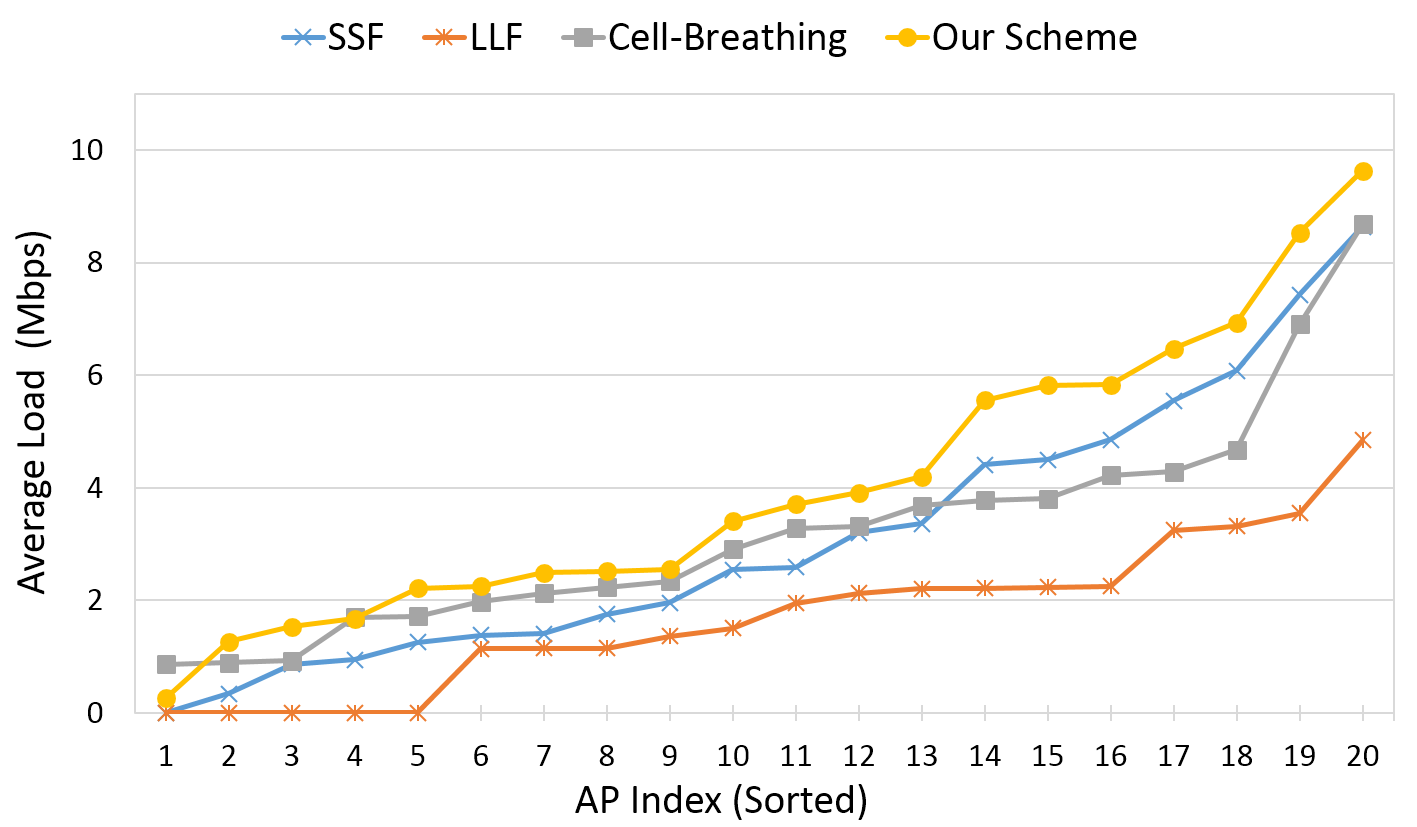
\includegraphics[width=3.4in]{images/Average_AP_load_400.png}
\end{center}
\caption{The Average Load of all APs (400 Users)}
\label{fig:fig4_2c}
\end{figure}

We calculate the average load of above three cases and compare the performance in Table \ref{tab:Total-AP-load}. As the population distribution becomes more crowded and imbalance (i.e. the number of users increases), the gap between our scheme and SSF is bigger. The load of our scheme performs $11\sim28\%$ better than SSF. Though the performance of Cell-Breathing becomes better in crowded and imbalance case, our scheme still performs $26\%$ better than Cell-Breathing. Figure \ref{fig:Total-AP-load} shows the total AP load during simulation time.

%% Table 4.3
\begin{table}[tbp]
\setlength{\belowcaptionskip}{15pt}
\centering
\caption{Summary of the AP load}
\label{tab:Total-AP-load}
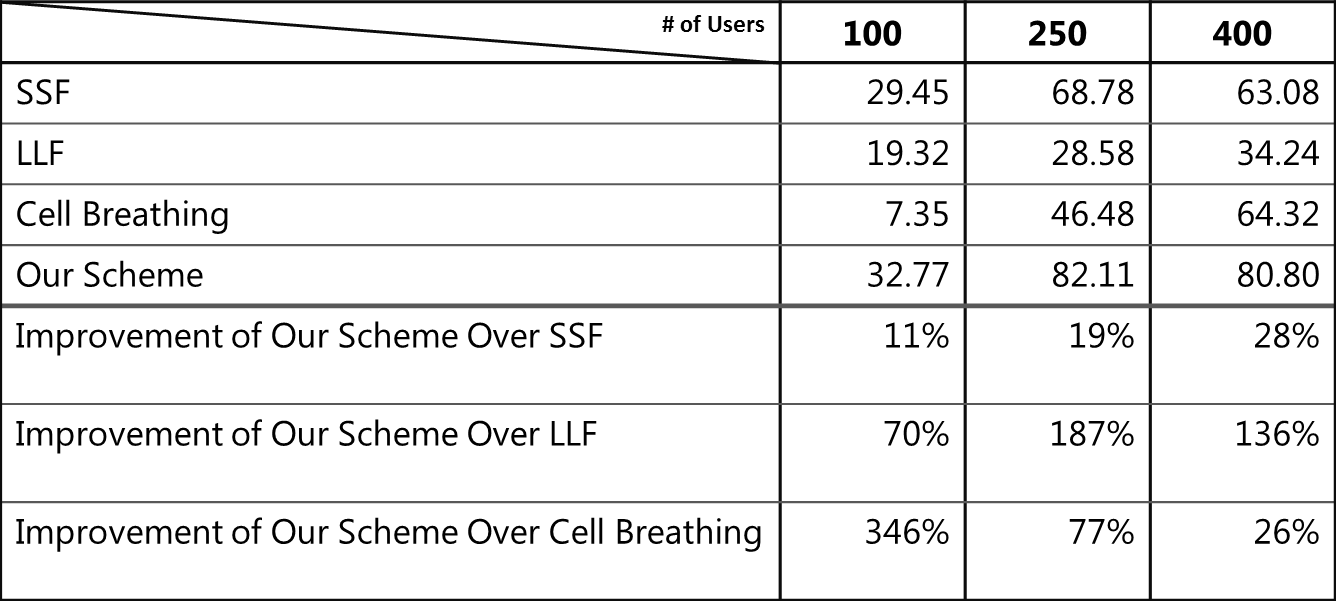
\includegraphics[width=3in]{images/table4_3.png}
\end{table}

%% Figure 4.3
\begin{figure}[tbp]
\begin{center}
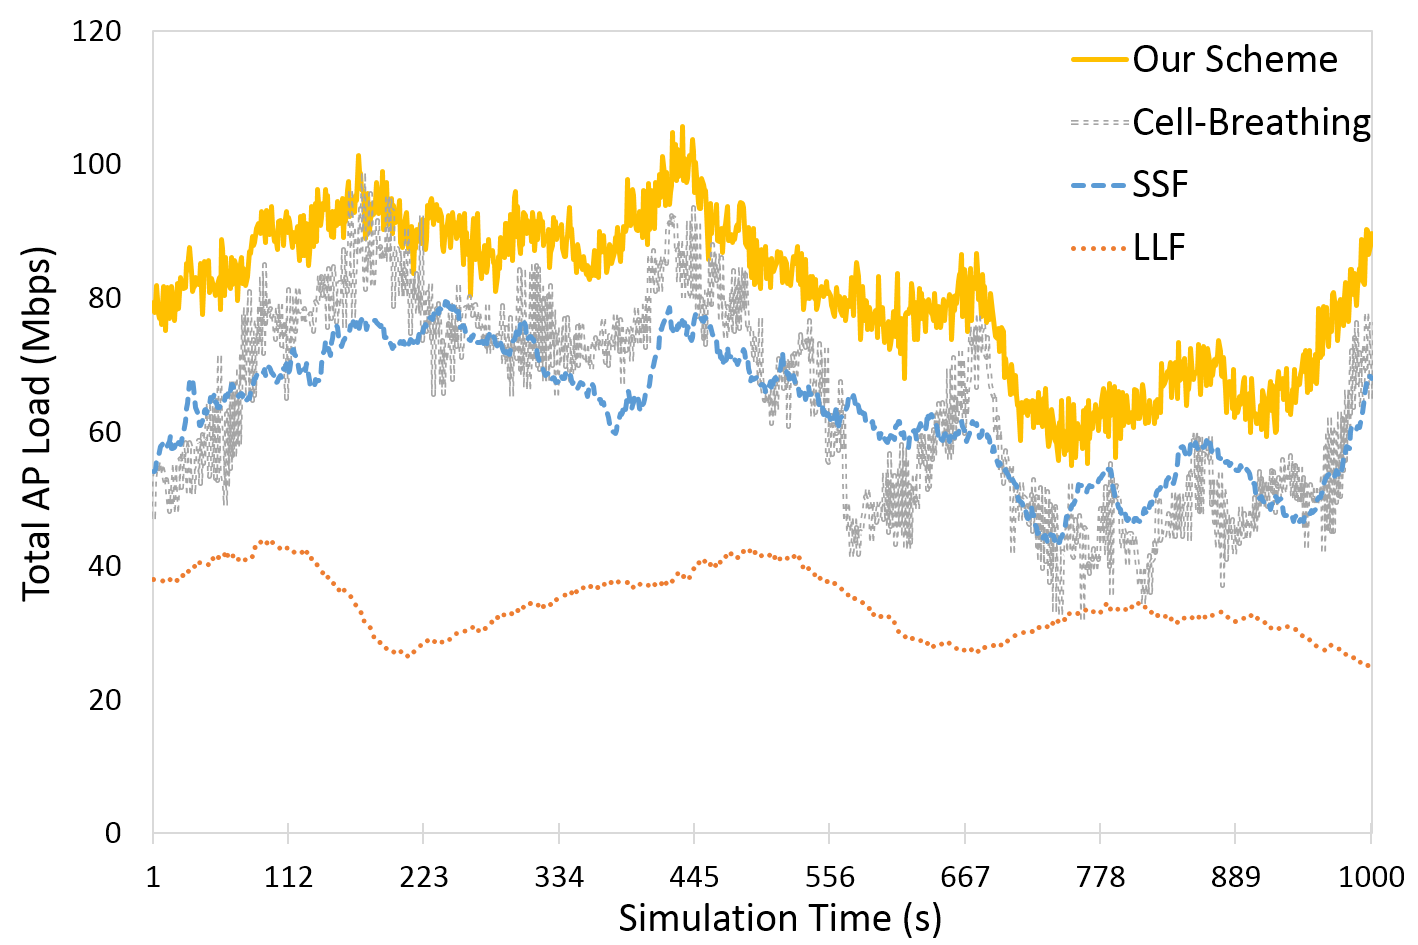
\includegraphics[width=3.4in]{images/Total_AP_load.png}
\end{center}
\caption{The Total AP Load (number of Users = 400)}
\label{fig:Total-AP-load}
\end{figure}

Figure \ref{fig:Average-user-number} illustrates the average user number of all APs in four methods. The X-axis represents the index of APs, and the APs are sorted by their average user number in increasing order. Our scheme and Cell-Breathing both balance the user number of all APs. SSF is the most imbalance method, because all users prefer to connect with the AP which has the strongest signal (i.e. the nearest AP). If there are too much users connecting to an AP at the same time, these users have poor bandwidth to transmit data.

%% Figure 4.4
\begin{figure}[tbp]
\begin{center}
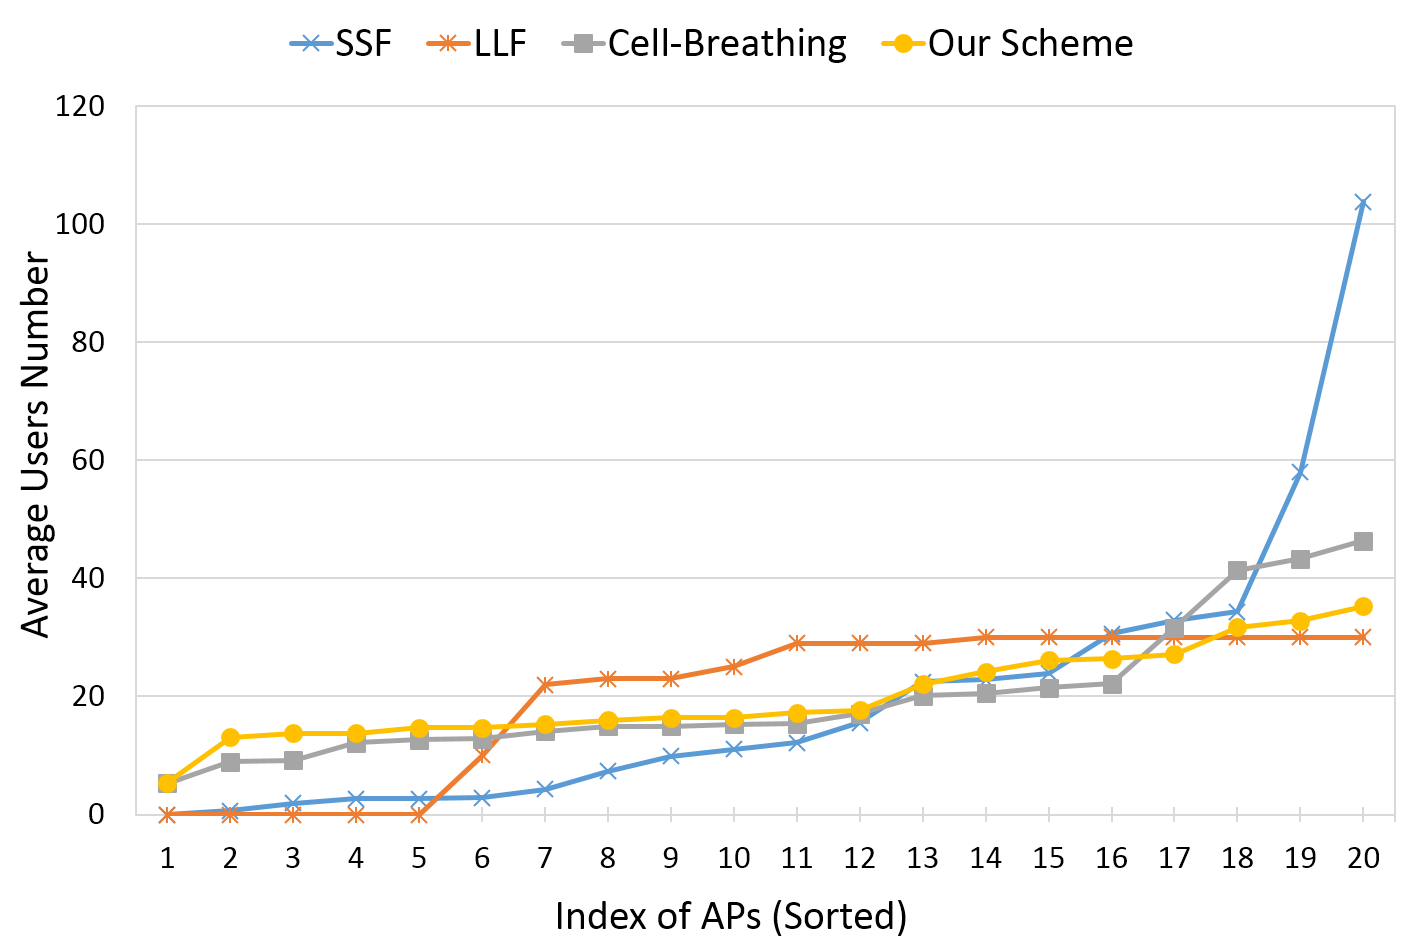
\includegraphics[width=3.4in]{images/Average_user_number.png}
\end{center}
\caption{The Average User Number of APs (number of Users = 400)}
\label{fig:Average-user-number}
\end{figure}
%\clearpage

\subsection{Impact of methods to Users}
In this subsection, we investigate the average user RSSI and average throughput with four methods. To measure the performance of user RSSI, we use the following formula and set Antenna gain 5 dBi.
\begin{equation}\label{RSSI}
  RSSI= Signal - Pathloss + Antenna_Gain
\end{equation}
In our simulation, we assume that the interference between adjacent APs can be ignored. We borrow the FSPL (Free Space Path Loss) equation of TP-Link to derive the path loss value.
\begin{equation}\label{Pathloss}
  Pathloss = 20log10(d)+ 20log10(f) + K
\end{equation}
$K$ is a constant number that depends on the unit used of distance $d$ and frequency $f$, and we set $K$ to 32.44 in our simulation.

Figure \ref{fig:Average-user-rssi} illustrates the average signal strength which user received from AP. The X-axis represents the index of users, and the users are sorted by their average RSSI in increasing order. Each average RSSI value is obtained from 10000 seconds. As a result, the users receive the highest average RSSI in SSF and the worst average RSSI in LLF. Since the users in SSF choose the highest RSSI AP to associate, and in LLF, the users intend to associate the lightest load AP. In Figure \ref{fig:Average-user-rssi}, the users in our scheme receive higher RSSI than the users in Cell-Breathing.

%% Figure 4.5
\begin{figure}[tbp]
\begin{center}
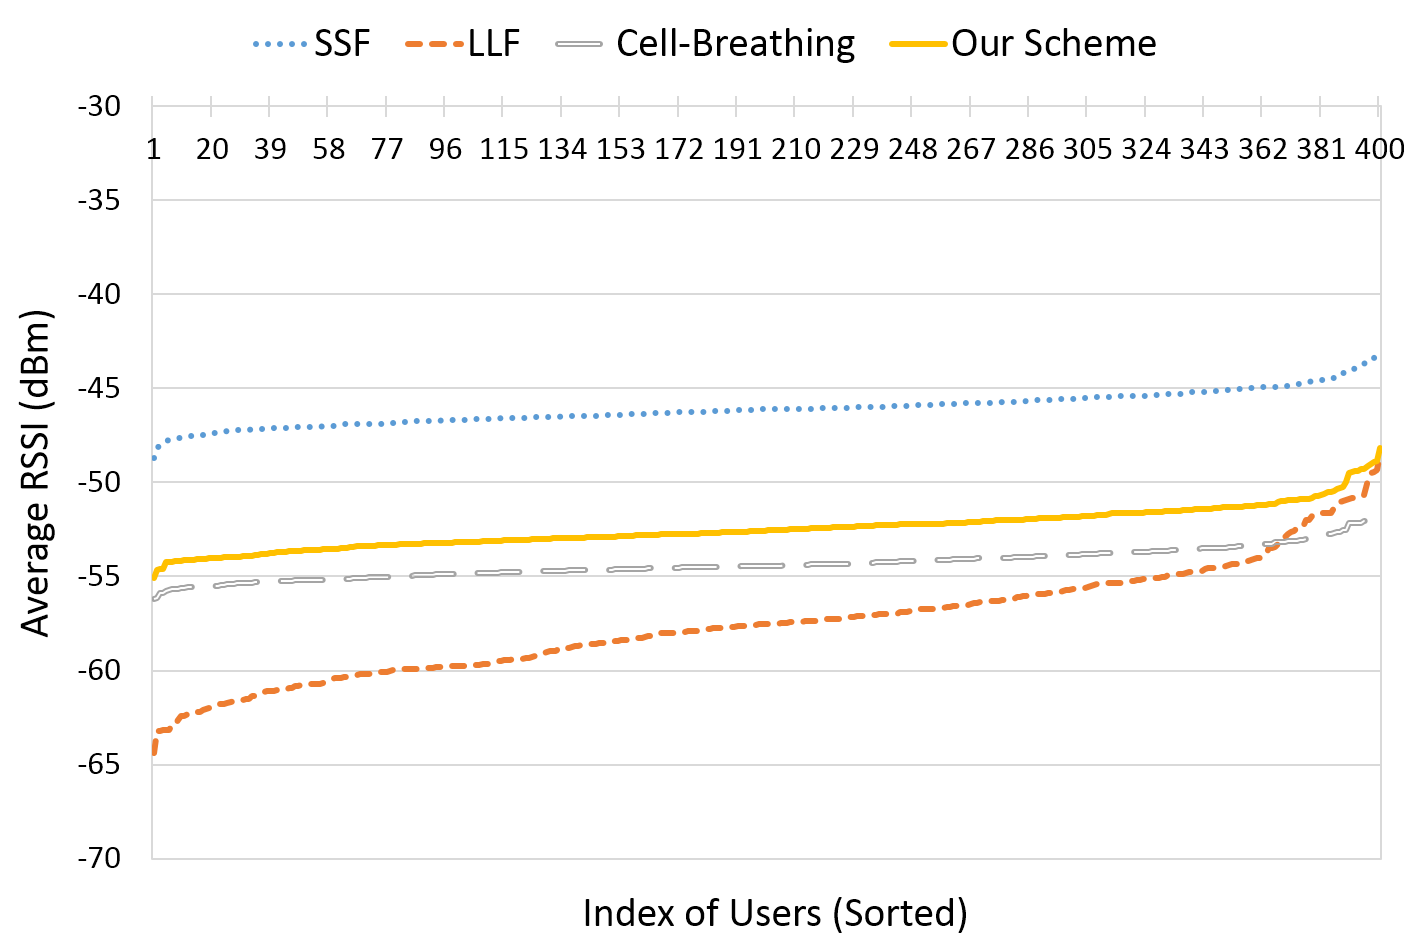
\includegraphics[width=3.4in]{images/Average_user_RSSI.png}
\end{center}
\caption{The Average RSSI of Users (number of Users = 400)}
\label{fig:Average-user-rssi}
\end{figure}

Figure \ref{fig:Average-user-throughput} shows the throughput of users. In our simulation, we assume that all users are “greedy” to use all the resource allocated from APs. However, the user usage is limited by not only user’s data rate but user’s bandwidth. In Figure \ref{fig:Average-user-throughput}, the users in our scheme have higher throughput than other methods. Due to our scheme shifts users from heavy load AP to light load AP, users can have better bandwidth and higher throughput.

We calculate the average throughput of three cases and compare the performance in Table \ref{tab:Average-user-throughput}. The load of our scheme performs $16\sim26\%$ better than SSF and performs $23\sim377\%$ better than Cell-Breathing. The performance of Cell-Breathing is very low when the population distribution is not too crowded. Overall, our scheme performs better than the other three methods in imbalanced and overcrowding environment.

%% Figure 4.6
\begin{figure}[tbp]
\begin{center}
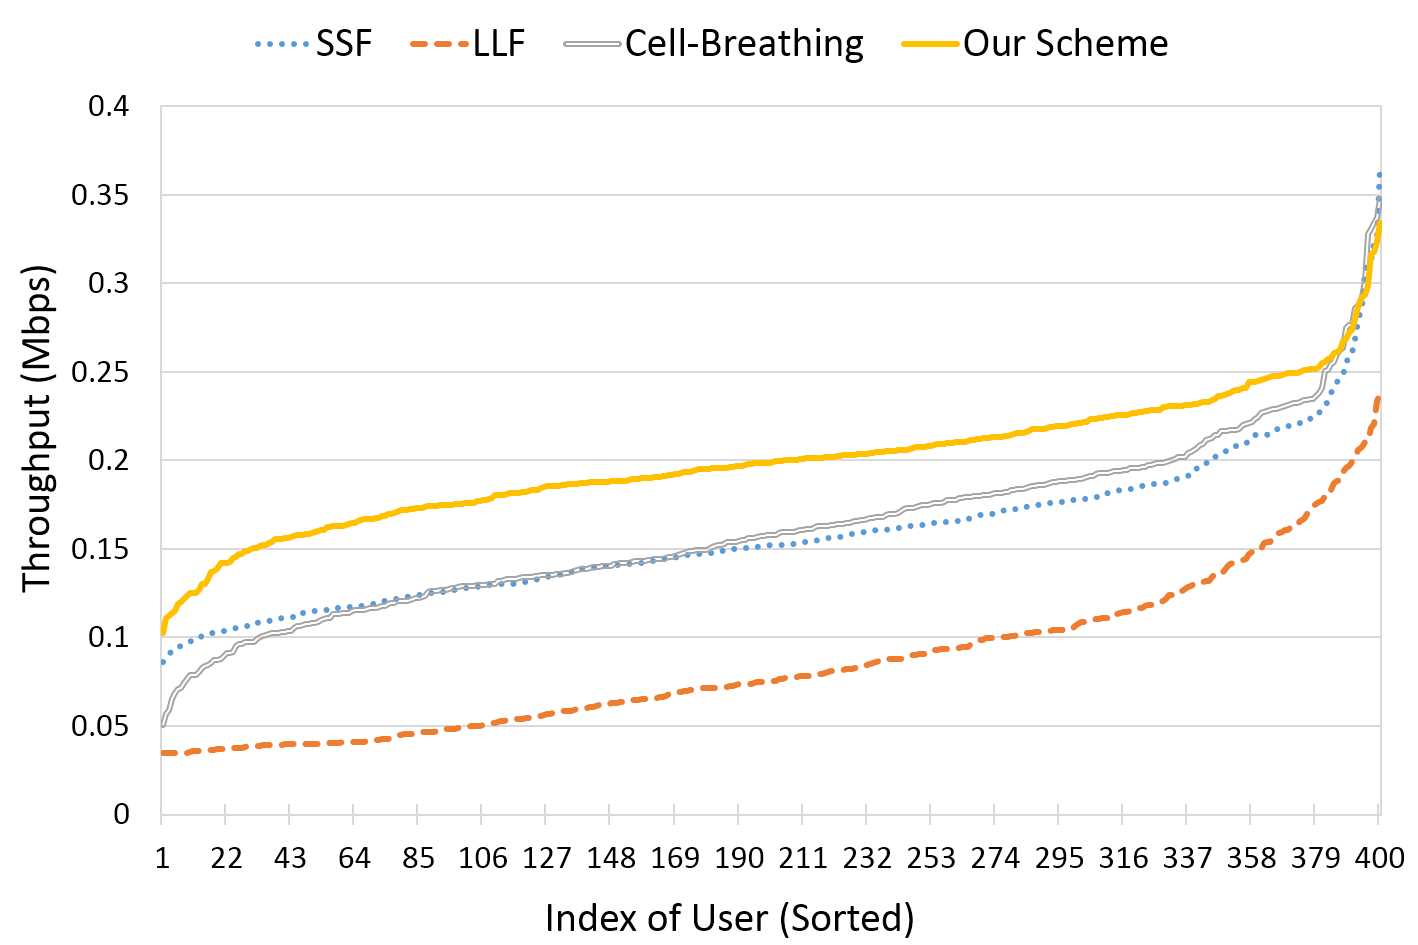
\includegraphics[width=3.4in]{images/Average_user_throughput.png}
\end{center}
\caption{The throughput of Users (number of Users = 400)}
\label{fig:Average-user-throughput}
\end{figure}

%% Table 4.4
\begin{table}[tbp]
\setlength{\belowcaptionskip}{15pt}
\centering
\caption{Summary of the User Throughput}
\label{tab:Average-user-throughput}
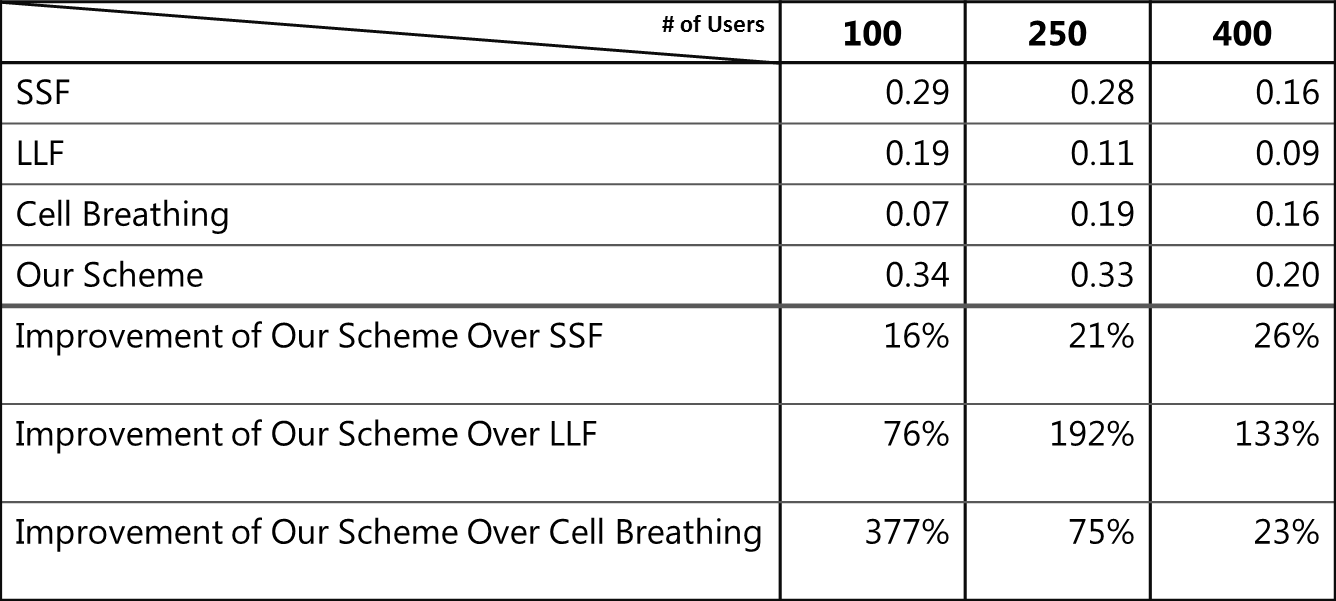
\includegraphics[width=3in]{images/table4_4.png}
\end{table}
%\clearpage

Figure \ref{fig:Levels} shows the impact of the power levels of our scheme. In the case of 400 users, these results show that the cases of more power levels perform better. Though the cases of more power levels take more time to compute the optimal solution, the computing time is much shorter than the people moving speed. In the figure \ref{fig:Levels}, the curve of 30 levels is almost overlapped with the curve of 50 levels, so we think that the power level ranging between 30 and 50 is suitable.

%% Figure 4.7
\begin{figure}[tbp]
\begin{center}
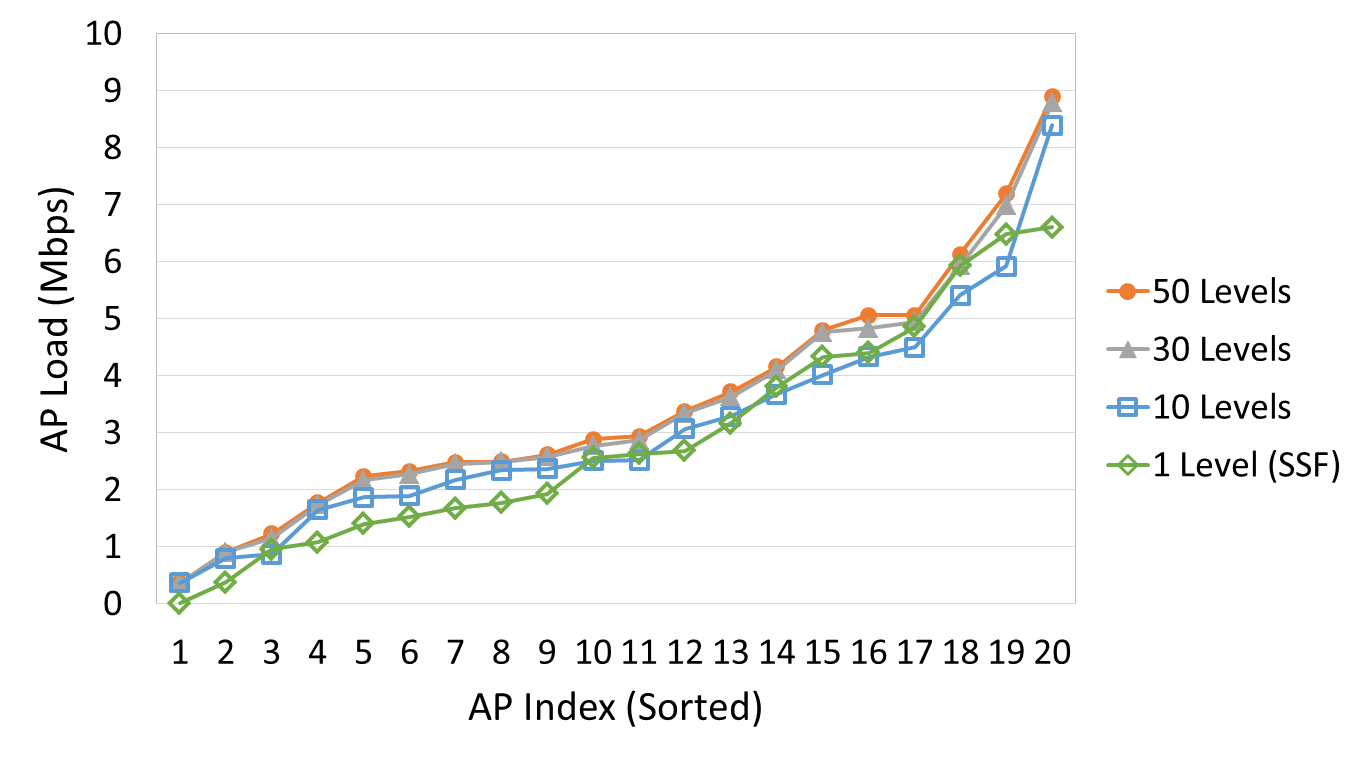
\includegraphics[width=3.4in]{images/Levels.png}
\end{center}
\caption{Impact of the Power Levels of Our Scheme}
\label{fig:Levels}
\end{figure}
% above dotto

	
\section{Conclusions} \label{ch:6-conclusion}
	%\hspace{24pt}
In this paper, we proposed an adaptive load balancing scheme through association control in wireless SDN. 
%We presented our system model as 
The proposed scheme consists of two parts: arrival event detection and adaptive load balancing. 
%In wireless SDN, we design the mechanism that 
Through SDN-based technique, APs report their load and connection situation to controller in real time. 
Based on the global vision of controller, we presented an algorithm on controller to derive the optimal association relationship between APs.
We compared the performance of the proposed scheme with SSF, LLF and Cell-Breathing methods through simulation experiments. 
The simulation results show that the average AP load of the proposed scheme is around 11 $\sim$ 28 \% higher than SSF and $26 \sim 346\%$ higher than Cell-Breathing. 
The proposed scheme checks AP load in real time and then shifts users from heavy-loaded APs to light-loaded APs, so that the total throughput is higher than that in other methods. 
Simulation results also show that the average user throughput of the proposed scheme is $16 \sim 26\%$ higher than SSF and $23 \sim 377\%$ higher than Cell-Breathing.



% use section* for acknowledgment
\section*{Acknowledgment}
%The authors would like to thank...
This work was sponsored in part by Ministry of Science and Technology (MOST), Taiwan, under the contract number MOST 105-2221-E-006-186-, MOST 105-2815-C-006-108-E, Industrial Technology Research Institute (ITRI) and Institute for Information Industry (III).

\bibliographystyle{IEEEtran}
\bibliography{reference}	
	
\end{document}

